\documentclass[11pt, a4paper] {report}
\usepackage[usenames,dvipsnames]{color}
\usepackage[pdftex,bookmarks=true]{hyperref}
\hypersetup{colorlinks=false,pdfborder={0 0 0 }}
\usepackage{url}
\usepackage{algorithmic}
\usepackage{algorithm}
\usepackage{graphicx}
\usepackage{amsmath}
\usepackage{subfigure}
\usepackage{verbatim}
\usepackage{moreverb}
\begin{document}
\begin{titlepage}
\begin{center}
\textsc{\Large Department of Computing\\Imperial College London}

\vfil

{\huge An A.I. Player for DEFCON:}\linebreak \linebreak
{\huge An Evolutionary Approach Using Behavior Trees}

\vfil

{\Large Final Year Individual Project}\linebreak \linebreak
{\Large Interim Report}\\[1cm]

{\large By: Chong-U Lim }

\vfil

{\Large Supervisor: Dr. Simon Colton} \linebreak \linebreak
{\Large 2nd Marker: Prof. Ian Hodkinson}

\vfil

{\large \today}

\end{center}
\end{titlepage}

% The abstract will go here
%\begin{abstract}
% As games become technologically more advanced with the ages, there's never been a greater need for intelligent AI in games. Several methodologies exist, with the aim of making AI more human-like, making games more engaging and believable. From the days of using Finite State Machines to Hierarchical Logic, the different ways of approaching AI have substantially made AI more diverse. Behavior Trees attempt to improve upon these techniques by allowing a modular, flexible and powerful architecture that is goal-orientated.  
%\end{abstract}

% The acknowledgements will go here
% \chapter*{Acknowledgements}

First of all, I would like to thank Professor Susan Eisenbach for supervising my project, and giving me invaluable advice and guidance throughout my work.

Secondly, I thank Dr. Tristan Allwood for his support, ideas, encouragement, and the useful discussions that we had regarding the direction of my project.

Also, many thanks to Chong-U Lim for his insight during our conversations, as well as to Yangfan Zhang, a close friend, without whom this project would not be what it is.

Finally, I would like to thank my family for their continued full support during the course of my university studies.


% Table of Contents
\tableofcontents


\setlength{\parskip}{0.2cm}

% Rest of Document

\chapter{Introduction}
This is the Report for my Final Year Project, \emph{Simple Python Lazy Automated Tester}, hence the acronym '\textsf{SPLAT}' appearing on the cover page, which represents the name of the tool created from this research.
%%%%%%%%%%%%%%%%%%%%%%%%%%%%%%%%%%%%%%%%%%%%%%%%%%%%%%%%%%%%%%%%%%%%%%%%%%%%%%%%%%%%%%%
\section{Motivation}	% describes the continual need for automated testing
Professional software engineers often write tests while developing code, especially for large complex codebases. These tests are highly beneficial for generating confidence in a bug-free solution delivery.

However, writing tests is not always easy to get right, and can be quite costly. It is reported that testing code is responsible for \emph{approximately half} the total cost of software development \cite{Edvardsson99asurvey}\cite{Han2008}\cite{Korel2005}.

Furthermore, this task becomes gradually more time-consuming as software grows in terms of complexity. Given similar resource constraints, it can become increasingly difficult to consistently achieve high test code coverage.

Moreover, a significant proportion of overall development time is spent writing test code not eventually included in production. Hence this work, though critical to assuring the quality of software \cite{Harrold00}, is ultimately invisible to the client, and sometimes difficult to justify this expenditure, as far as billing and accountability is concerned.

This has led to a large body of work on automatically generating unit test suites, particularly notable within the imperative programming community \cite{Allwood2011}, in order to reduce the effort of unit testing required, to encourage wider adoption by developers.

Even then, the present need for manual testing indicates that there still remains much scope for improvement. A recent example supporting this claim is Google handing out a record \$26k in bug bounties for security researchers reporting Chrome vulnerabilities \cite{ChromeBugBounties}.

Therefore, this example raises the question of whether full automatic discovery \cite{Bertolino2007} for all these bugs could be possible, in order to eliminate the cost of manual testing, let alone any bug exploits.
%%%%%%%%%%%%%%%%%%%%%%%%%%%%%%%%%%%%%%%%%%%%%%%%%%%%%%%%%%%%%%%%%%%%%%%%%%%%%%%%%%%%%%%
\section{Automated software testing for dynamic languages}
Whilst research in this field is typically devoted to statically typed programming languages such as C/C++, Objective-C or Java/Scala, relatively less emphasis is placed on their dynamic counterparts like Javascript, Python or Ruby.

This observation is made in contrast to the rapid growth in popularity of dynamic languages in recent years, especially Python. Python was named the `The Importance Of Being Earnest' (TIOBE) Programming Language of the Year, both in 2007 and 2010 \cite{TiobeDec11}. Therefore, Python is the subject of this paper.

One paper implements the search-based software testing (SBST) technique, to automatically generate test scenarios for Ruby code, using genetic algorithms \cite{Mairhofer2011}. There is neither any equivalent tool targeting Python however, nor any chance of porting these tests for Python programs.

In that paper, the authors claimed success in achieving consistent and significantly high code coverage over a preselected set of test inputs with their tool, when compared against the \naive random test case generator. Would it be possible to improve this using a suitable adaptation of existing techniques, and/or to maintain this coverage across a more extensive range of programs written for different problem domains?

As Python, like Ruby, is a reflective, dynamically typed language, it would seem logical to adopt a similar approach in solving this problem, specifically by generating test scenarios via \emph{runtime code analysis} \cite{Mairhofer2011}.
%%%%%%%%%%%%%%%%%%%%%%%%%%%%%%%%%%%%%%%%%%%%%%%%%%%%%%%%%%%%%%%%%%%%%%%%%%%%%%%%%%%%%%%
\section{The Python programming language}
Growing numbers of commercial and closed source applications are being developed using the Python programming language \cite{Smith2011}. Hence, this project would also be looking at automatically generating unit tests for Python bytecode, instead of from Python source code traditionally.

The Python programming language contains a variety of interesting features which encourage rapid experimentation with automatic testing techniques. This is primarily because Python is an open source, general purpose, multi-paradigm, cross-platform compatible, dynamically typed language, offering duck typing, and in active development and support. It also provides \emph{excellent builtin introspection and reflection capabilities}, to inspect and manipulate code at runtime.

At the heart of the language design philosophy \cite{Pep20ZenPython}, there should be one -- and preferably only one -- obvious way to do things. The importance of readability promotes a \emph{clean, concise and elegant syntax}, which makes demonstrating 'proof of concept' code easy.
\clearpage
For instance, the following Python code snippet certainly reads more fluently than its C\# counterpart:

\begin{tabularx}{\textwidth}{X X}
\underline{Sample C\# code} & \underline{Equivalent Python code} \\
\begin{lstlisting}[language=CSharp]^^J
if ("hello".indexOf("e") >= 0)^^J
\{^^J
\ \ \ return true;^^J
\}^^J
\end{lstlisting}
&
\begin{lstlisting}[language=python]^^J
if 'e' in 'hello':^^J
\ \ \ return True^^J
\end{lstlisting}
\end{tabularx}
Python features a fundamental testing infrastructure toolset based on \textsf{unittest}, \textsf{doctest} and \textsf{py.test}. However, there is limited availability of testing support tools built on top of those. Many of these either target outdated versions of Python, or are discontinued. There are a few candidate tools for automated testing, for instance, \textsf{pythoscope} and \textsf{pytestsgenerator}, which generate tests by performing static code analysis. However, there are no tools which perform dynamic test case generation.
%%%%%%%%%%%%%%%%%%%%%%%%%%%%%%%%%%%%%%%%%%%%%%%%%%%%%%%%%%%%%%%%%%%%%%%%%%%%%%%%%%%%%%%
\section{Project contributions}
Within the context given above, this project makes the following key contributions:

\begin{itemize}
	\item A discussion of the possible ways considered for automated software testing, focusing on test data generation by using information gathered at runtime
	\item A motivating example describing automated lazy testing in Python
	\item Implementation as a Python module, to automatically generate consistently high coverage test suites, primarily evaluated against Python libraries like python-graph, and other Python module implementations of famous algorithms
	\item Investigating effectiveness of the \emph{lazy instantiation} testing technique, as illustrated by \textsc{Irulan} in Haskell \cite{Allwood2011}, for Python
	\item Further advance the work in the field of automated software testing, especially for dynamic languages
\end{itemize}

To this end, we take advantage of the main features of the core Python language, ie. \emph{strong introspection and reflective capabilities}, combined together with its extensive tool support from the Python Package Index (PyPI) repository.
\clearpage
The concepts discussed in this paper are concretely demonstrated in a tool called \textsc{Splat}, a high coverage test suite generator for Python modules, written in Python, but portable to target other languages. This tool has been successfully applied to some of the most popular frameworks, achieving the initial objective of consistently high test code coverage, comparable to those manual unit tests written by hand, and even potentially discovering several bugs in the process as well. The tool has also been extended to support regression testing, where reports on a sample of case studies are included in this report.

\section{Report organisation}
Firstly, relevant background material is reviewed in Chapter \ref{ch:background}. Thereafter, the various algorithms and techniques used to automatically generate tests are formally introduced in Chapter \ref{ch:contrib}. These ideas presented are then implemented in the tool \textsc{Splat}, constituting the subject of Chapter \ref{ch:splat}. This is accompanied by a detailed description of \textsc{Splat}'s software design architecture, together with several worked examples, for clarification purposes. A summary of the extent of success of the project is discussed in Chapter \ref{ch:eval}. Lastly, some final conclusions are drawn, before suggestions are given to possible future work in Chapter \ref{ch:conclusion}.

\chapter{Background}
    
\textbf{\LARGE{Overview}}

In this chapter, we present information from various sources that provide a deeper understanding of certain methodologies, applications and technical information pertaining to this project. For the purpose of this interim report, in addition to the details of the background topic, suggested applications of each of these topics for the purpose of this project are also presented.

In Section~\ref{sec:defcon}, we introduce the commercial real-times strategy game DEFCON covering gameplay, game rules and coverage of existing AIs that have been developed for the purpose of automating the playing of DEFCON.

In Section~\ref{sec:behaviortrees}, we introduce the design and usage of Behavior Trees - a hierarchical structure used to encode AI. We go over what defines a behavior tree, its composition and run through various examples of the usage of different types of behavior trees. 

In Section~\ref{sec:bod}, Behavior-Oriented Design (BOD) is introduced as a programming methodology to approaching AI design. We introduce the motivation and proposed design process, and also present our proposed approach to using Behavior Trees to make use of this design methodology.

In Section~\ref{sec:ga}, we cover Genetic Algorithms as a Machine Learning technique, covering its definition and operators, and also present our proposed approach to its application to Behavior Trees.

    \newpage
    
    \section{Defcon}
    \label{sec:defcon}
        DEFCON is a multiplayer real-time strategy game that allows players to take the roles of the military commanders of one of six possible world territories. Players are given a set of units and structures at their disposal, and it is up to them to manage these resources and inflict the biggest amount of damage against opposing players. The game is split into 5 discrete intervals, named from DEFCON5 to DEFCON1, and these intervals dictate the possible movements and manipulation of units. 
        
        It's described as a \emph{genocide}-em-up, a play on the term \emph{shoot}-em-up and \emph{beat}-em-up often used to classify other game genres such as first-person-shooters and action games respectively, and since a large element of the game of DEFCON involves the use of nuclear missles to annihalate large populations of opponent players. Battles are fought in sea and air, and the game involves strategic planning and decision making in coordinating all these units in order to win. Figure~\ref{img:defconss} shows an in-game screenshot of a coordinated attack in DEFCON, taken from DEFCON's official website~\footnote{Introversion Software's Official DEFCON Site: http://www.introversion.co.uk/defcon/}.
        
        \begin{figure}[htp]
            \begin{center}
            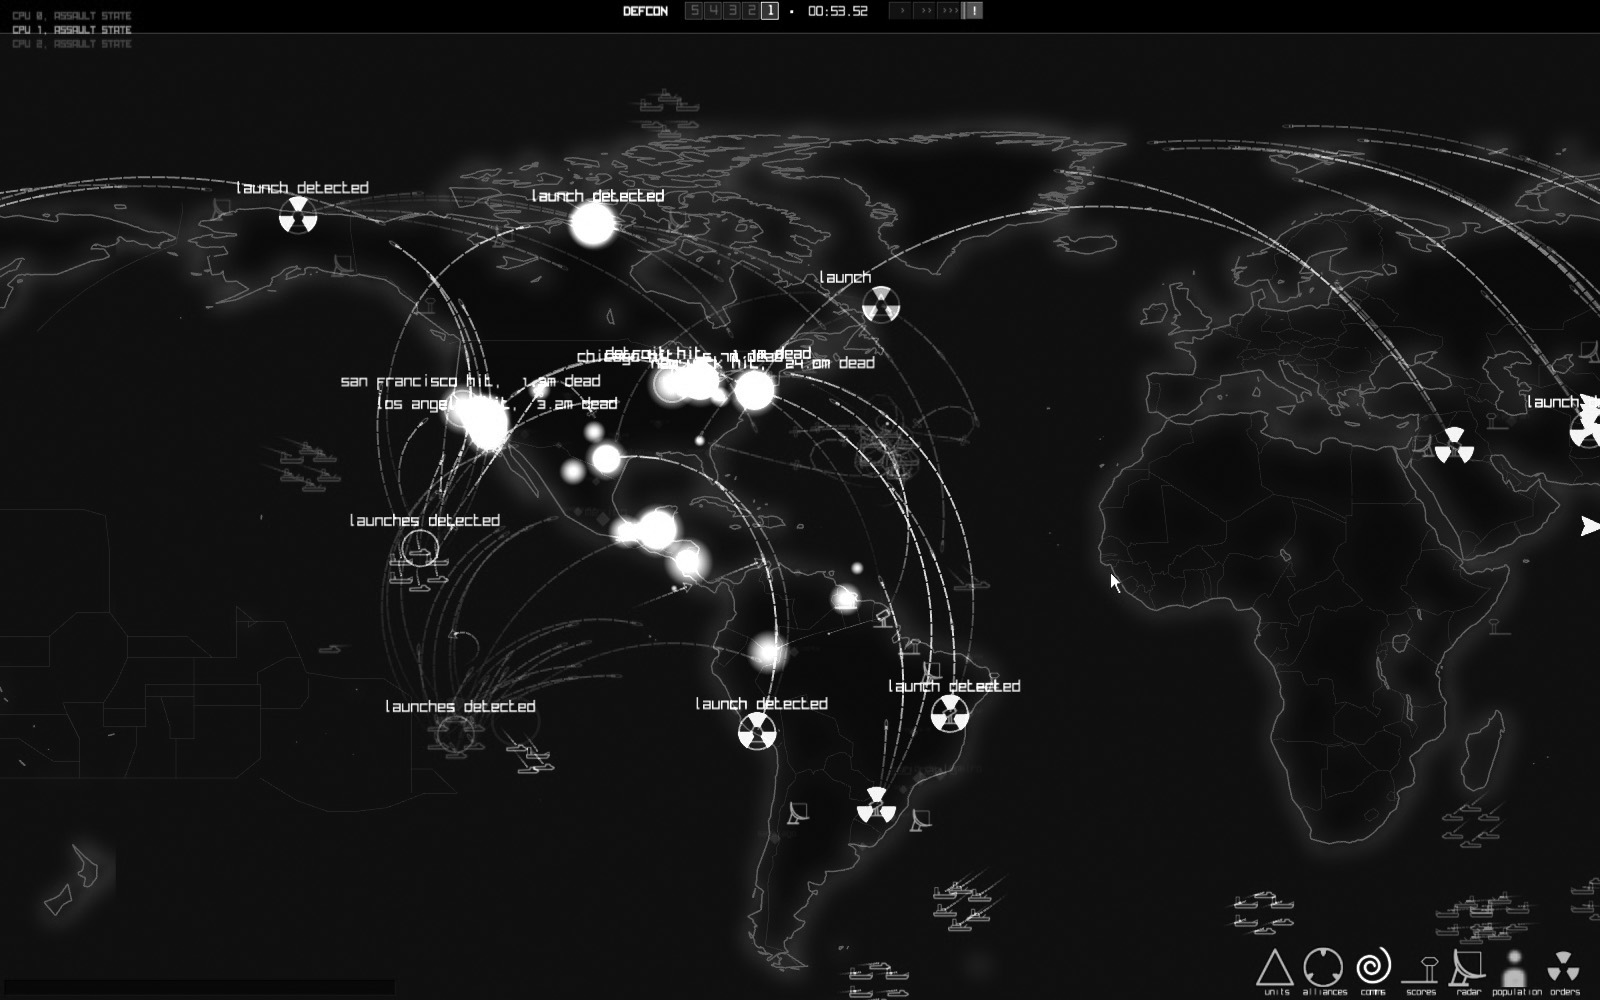
\includegraphics[scale=0.2]{images/defconss.jpg}
            \caption{Global conflict erupts with a series of co-ordinated strikes in Defcon}
            \label{img:defconss}
            \end{center} 
        \end{figure}
        
        In this section, we begin by covering an overview of the game of ~DEFCON, covering basic game rules and gameplay elements.  We proceed to present existing AIs which are presently available. Finally, we briefly cover the DEFCON API which is being used for the purpose of developing an AI for this project.
              
        
        \subsection{Overview}       
        
        The information here has been consolidated from both the official DEFCON manual\footnote{Available at the official website} and Robin Baumgarten's Thesis "Automating the Playing of DEFCON"~\cite{robbot}
        
        \subsubsection{Parties \& Territories} 
        
        A \textbf{party} represents the player, either human or AI-controlled, in the game of DEFCON. As such, there are at least 2 parties in the game. Each party is assigned a \textbf{territory} at the start of a DEFCON match, and this allocation is either done randomly or chosen.
         
        There are 7 available \textbf{territories} in each game, and each territory is controlled by up to 1 party. As such, in a game involving two players, two territories will be controlled by one player, and the remaining five territories will remain unassigned to any party. Each controlled territory possesses at least one \textbf{city}, and each city consists of a non-negative number representing its population. The total sum of the population for each territory is equal between all 7. The territory designates the points on the map that a player may place \textbf{land units} and each player may only do so in his or her respective territories.
                          
        A portion of the sea, \textbf{sea-territories}, are associate with each party whereby \textbf{navy units} may be placed in.       
        
        \subsubsection{Units}
        Each party is allocated a fixed quantity of units that it may place and make use of throughout the course of the game. Each unit possesses one or more states which indicate the type of actions is may execute. The units are classified into 3 groups, namely,

        \begin{itemize}
        \item Ground Installations
        \item Navy Units
        \item Aerial Units
        \end{itemize}
         
        \paragraph{Ground Installations}
        
        \begin{itemize}
        \item \textbf{RadarStation}: Radars scan a wide range and display enemy units within their range on the map.
        \item \textbf{Silo}: Silo contains 10 Long Range Ballistic Missiles (LRBMs) and can take 3 direct hits before it is destroyed. A Silo has two modes: 
            \begin{itemize}
               \item \textbf{Nuclear Launch}: A target on the map may be manually selected to launch a missle. Upon launch, it can not defend itself, and reveals its position to other players after launching its missiles. 
               \item \textbf{Air-Defense}: Enemy airforce units and nukes in range are automatically attacked, in the decreasing priority of Nukes over Bombers over FIghters. If there are several of the same class, it chooses the closest. 
            \end{itemize}
        \item \textbf{Airbase}: Starts with 5 bombers, 5 fighters and 10 Short Range Ballistic Missiles (SRBMs) by default. An Airbase has two modes:
            \begin{itemize}
            \item \textbf{Launch Fighters}: A target within range may be targetted, in which Fighter units are launched. The recharge time after the launch of a Fighter, whilst no other Fighters can be launched is 20 seconds.
            \item \textbf{Launch Bombers}: A target within range may be targetted, in which Bomber units are launched. The recharge time after the launch of a Bomber, whilst no other Bombers can be launched is 20 seconds.
            \end{itemize}
        \end{itemize}
         
        \paragraph{Air Forces}

         \begin{itemize}
         \item \textbf{Fighter}: Fighters may attack other Fighters and Bombers, and may used for scouting to discover enemy installations. A Fighter has limited fuel, and automatically return to any Airbase or Carrier upon completion of objective, otherwise it will crash and is lost.
         \item \textbf{Bomber}: Bombers carry a single Short Range Ballistic Missle (SRBM), and can be used to fly and deploy nukes at close range. A Figher has two modes:
            \begin{itemize}
               \item \textbf{Naval Combat} Attacks visible enemy Navy units.
               \item \textbf{Missle Launch} A target may be targetted to launch a misle against.   
            \end{itemize}
         \end{itemize}    

        \paragraph{Navy Units}
        \begin{itemize}
         \item \textbf{Carrier}: Starts with 5 fighters, 2 bombers and 6 SRMBs. Can also launch depth charges against submarines in the vicinity. It consists of 3 modes:
            \begin{itemize}
               \item \textbf{Fighter Launch}: Hostile units within range may be targeted and Fighters are launched.
               \item \textbf{Bomber Launch}:  Hostile units within range may be targeted and Bombers are launched.
               \item \textbf{Anti-Submarine}: A sonar scan is performed, and enemy submarines within range are revealed, where a depth charge is released. 
            \end{itemize}.  
         \item \textbf{Battleship}: Battleships can only attack with conventional weapons,however they are extremely effective against other naval units and aircraft.
         \item \textbf{Submarine}: Submarines contain 5 Medium Range Ballistic Missiles(MRBMs) and are either submerged or surfaced. They are invisible to radar while submerged, but must surface to launch. They can be detected by sonar pings from carriers or other subs. Once detected or surfaced they are very vulnerable to attack. It has 3 modes:
            \begin{itemize}
               \item \textbf{Passive-Sonar}: Submarine remains invisible to radar and can only be detected by carriers in anti submarine status and other submarines in active sonar mode. It can attack hostile naval units if they are visible to the party of the submarine.

               \item \textbf{Active-Sonar}: Similar to Passive-Sonar, except in addition, Submarine creates a sonar scan, which reveals all naval units within a certain distance from the submarine. 

               \item \textbf{Launch Missle}: A target within range may be attacke, where a missle is launched. In this state, the submarines surfaces and is no longer invisible until all its missles have been depleted whereby it returns to Passive-Sonar mode.
            \end{itemize}
         \end{itemize}
        
        \newpage
        
        \subsubsection{Defcon Levels}
        The course of the game of DEFCON spans over the couse of 5 DEFCON phases, starting from DEFCON5. In each DEFCON phase, certain actions and information are permitted whilst others are not. Table~\ref{tab:defconlevels} gives an explanation of each of the DEFCON phases and a description of what is involved in each.
             
        \begin{center}
        \begin{figure}
        \begin{center}
        \begin{tabular}{ | p{2cm} | p{7cm}| p{1.5cm} | }
        \hline
        \textbf{Defcon Level} & \textbf{Description}  & \textbf{Time} \\ \hline \hline        
        5 & No hostile actions. Ground installations may be placed. Fleets may be placed and moved within international waters & 3 \\ \hline
        4 & Radar coverage will provide information on enemy units if within range & 3 \\ \hline
        3 & Units and ground installations may no longer be placed. Naval and Air attacks not involving Missles are permitted & 3   \\ \hline
        2 & This is essentially the same as in DEFCON 3 & 3 \\ \hline
        1 & No units may be placed, and missle attacks are now allowed. This phase continues until 80\% of all missles in the game has been launched, after which a victory timer counts down until the end of the game. & -  \\ \hline
        \hline        
        \end{tabular}
        \caption{Summary of DEFCON levels and permitted actions}
        \label{tab:defconlevels}
        \end{center}
        \end{figure}
        \end{center}
        
        
        \subsubsection{Winning Conditions}

        Winning in the game of DEFCON involves attaining the higest score, and how these scores are calculated differently according to the \emph{Scoring Mode} which is decided at the start of a game. The 3 modes are:

         \begin{itemize}
         \item \textbf{Default}: 2 points awarded for every million of the opponent's people killed. -1 point penalty for every million people belonging to the player.
         \item \textbf{Genocide}: 1 point is awarded for every million of the opponent's people killed. No penalty for losing a player's own people.
         \item \textbf{Survivor}: 1 point is awarded for every million people surviving in the player's territory. The points start at 100 for both teams and decrease throughout the game.
         \end{itemize}    
        
        \pagebreak
        
        \subsection{AI in DEFCON}
        \label{sec:defcon-bots}
        Several implementations of AIs have been created for the puporse of automating the playing the game of DEFCON. These implementations of AI-controlled players are often referred to as \textbf{bots}\footnote{For the purpose of this report, the term \textbf{bot} is used to refer to any AI-controlled player in DEFCON}, or \textbf{CPU Players}.
        
        We cover two such bots in this section, namely the default bot that ships together with the game which allows human players to pit themselves against an opponent without the need for a network connection with another human player. The second is the result of a Master's thesis by Robin Baumgarten~\cite{robbot}, which was developed using a combination AI machine learning techniques.
        
        \subsubsection{Introversion Bot}
        The default bot\footnote{Henceforth termed as the Introversion Bot} that comes with DEFCON is a deterministic, finite-state-machine driven bot~\cite{robbot}. It consists of a set of 5 states and transits from one state to the next in sequence. Upon reaching the final state, remains in it until the end of the game. This is depicted in Figure~\ref{img:defaultbot}, The states and a brief description, as identified by Baumgarten~\cite{robbot} of what occurs in each are:
        
        \begin{figure}[htp]
            \begin{center}
            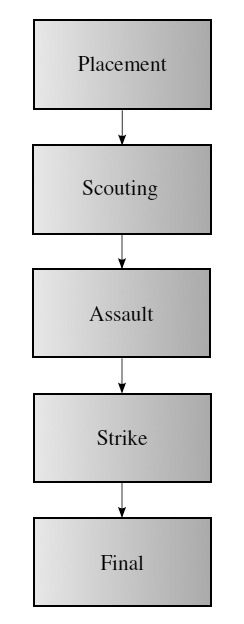
\includegraphics[scale=0.4]{images/defaultbot.png}
            \caption{Sequence of States in Introversion Bot}
            \label{img:defaultbot}
            \end{center} 
        \end{figure}
        
        \newpage
        
        \begin{itemize}
        \item \textbf{Placement}: Fleets and structures are placed. The fleet is randomly placed at predefined starting positions. Structures are placed near cities. Once all units are placed, the AI proceeds to the next state.
        \item \textbf{Scouting}: The AI tries to uncover structures of a random opponent by moving fleets towards occupied territories and launching fighters towards them. Once 5 structures have been uncovered or a predefined assault timer 10 expires or the victory timer starts the next state is invoked.
        \item \textbf{Assault}: The AI starts to launch missile attacks with bombers and subs on the previously chosen opponent. Once 5 structures have been destroyed or the assault timer expires or the victory timer starts, the strike state is invoked.
        \item \textbf{Strike}: Silos launch their missiles and other missile carrying units continue to attack. After these attacks have been initiated, the system changes into the final state.
        \item \textbf{Final}: In the final state no more strategic commands are issued. Fleets continue to approach random attack spots.
        \end{itemize}
        
        \subsubsection{Robin's Bot}
        \label{sec:robbot}

        In 2007, a bot was developed by Baumgarten~\cite{robbot} using a combination of AI machine learning techniques such as case-based reasoning, decision tree algorithms and hierarchical planning\footnote{Henceforth referred to as Robin's Bot}. For the case-based reasoning system, high-level strategy plans for matches were automatically created by querying a case base of recorded matches and building a plan decision tree. A broad overview of the system design is depicted in Figure~\ref{img:robbot-design}. 
        
        \begin{figure}[htp]
            \begin{center}
            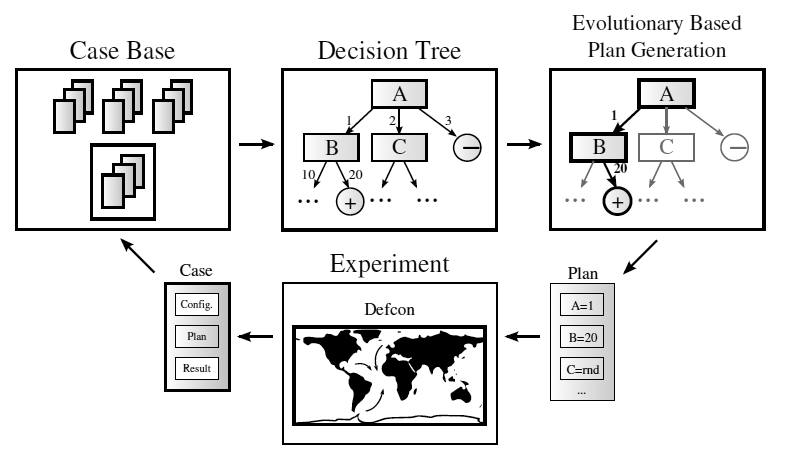
\includegraphics[scale=0.4]{images/robbot-design.png}
            \caption{Overview of System Design in Robin's Bot}
            \label{img:robbot-design}
            \end{center} 
        \end{figure}
        
        
        \newpage
        
        The implementation of the bot can be described as a series of steps:
        
        \begin{enumerate}
        \item At the start of the game, territories are assigned randomly to both the Introversion Bot and Robin's bot
        \item Upon assignment, the starting configuration is used as similarity measure to retrieve a case from the case-base
        \item Plans from the retrieved case classified into a decision tree with plan attributes
        \item The decision tree determines a high-level plan coordinating groups of fleets, termed metafleets, and are placed as dictated by the plan.
        \item The placement of structures is controlled by an algorithm taking recent matches into account by querying the case base
        \item With everything placed, an attack on the opponent's mainland is prepared establishing where and when to attack
        \item A synchronised attack is performed, and the game ends
        \item Results, the plan used, fleet movement and structure information  are extracted into the case and retained in the case base.
        \end{enumerate}        
        
        \subsection{DEFCON API}   
        Funded by a Technology Strategy Board feasibility study grant, via a partnership of Introversion Software and Imperial College, Imperial College has developed an Advanced Programming Interface (API) for Introversion's DEFCON game~\footnote{API and documentation available from http://www.doc.ic.ac.uk/~rb1006/projects:api}. The API provides an interface to DEFCON's methods and function calls, and is used to produce a dynamic-link library (.dll) file that contains an AI implementation which can be then included as a module for DEFCON to access and use as an AI player.

        The API provides a way for AI developers to develop AI bots for the game of DEFCON, without having to work with the source-code of DEFCON directly, expanding its reach to people to give a shot at developing an AI for DEFCON. At the time of writing, the API is at version 1.51, and provides the base framework for which this project is based on. By making use of the API to develop the bot, we hope to progressively contribute ideas and improvements to the API together with advances in this project.       
    
    \newpage
    
    \section{Behavior Trees}
    \label{sec:behaviortrees}
        
        Behavior Trees represent a new way of defining the AI for video games. Its key characteristics are being simple to define, scalable to exhibit complex AI and modular for reusability~\cite{understandingbts}. This is achieved by introducing a set of constructs which a Behavior Tree is essentially composed of in the form of nodes. Behavior Trees are essentially goal-oriented, with each tree associated with a distinct, high-level goal which it attempts to achieve. Behavior Trees can be linked together, allowing the exhibition of complex behaviors by first defining smaller, sub-behaviors. 
        
        In this section, we take a look at the motivation for Behavior Trees, making comparisons to other traditional forms of defining game AI used in practice. We then cover the 5 basic constructs that are used to create Behavior Trees. Following that, we discuss the goal-oriented design of Behavior Trees and finally, a discussion on how this enables Behavior Trees to perform planning to achieve these goals.
        
        We have adopted a similar convention for the style and design representing the types of nodes in Behavior Trees from Alex J. Champandard's presentation on Behavior Trees~\cite{btnextgenpart1}
       
        \subsection{Motivation}
        
        A traditional approach to developing AI for games has been to use Finite State Machines (FSM).  To illustrate this, we use the following diagrams and example regarding the AI for a simple service robot from Ian Millington's Artificial Intelligence for Games~\cite{millington}. 
        
        \begin{figure}[htp]
            \begin{center}
            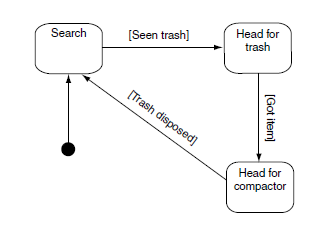
\includegraphics[scale=0.5]{images/fsm1.png}
            \caption{Basic FSM of a cleaning robot}
            \label{img:fsm1}
            \end{center} 
        \end{figure}
        
        Figure~\ref{img:fsm1} illustrates the FSM for a the AI of simple service robot, and how a FSM handles its abilities to  search around for objects that have been dropped, pick one up when it finds it, and carry it off to the trash compactor. Now consider Figure~\ref{img:fsm2}, whereby the robot now has an alarm system to indicate whether its power is running low.

        \begin{figure}[htp]
            \begin{center}
            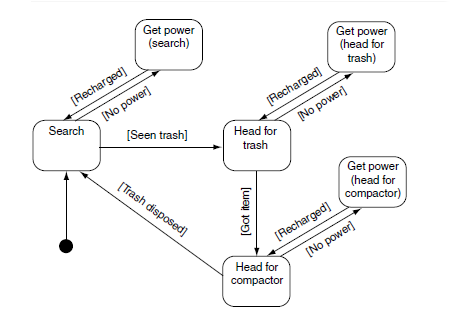
\includegraphics[scale=0.5]{images/fsm2.png}
            \caption{Extended FSM of a cleaning robot}
            \label{img:fsm2}
            \end{center} 
        \end{figure}
        
        It can be seen that the number of states have now doubled in order to accomodate this new functionality. Thus, it can be seen that if the subject grows in complexity, the number of states that are required to represent the AI logic increases, along with the transitions between the states. This led to the introduction of Hierarchical Finite State Machines (HSFMS), which were introduced to overcome these drawbacks, improving scalability by grouping states to share these transitions to develop larger and more complex AI systems. This is illustrated in Figure~\ref{img:hfsm}. 
                      
        \begin{figure}[htp]
            \begin{center}
            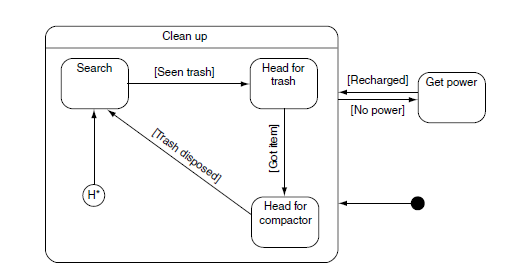
\includegraphics[scale=0.5]{images/hfsm.png}
            \caption{Hierarchical FSM of a cleaning robot}
            \label{img:hfsm}
            \end{center} 
        \end{figure}

       However these numerous transitions still have to be defined carefully in order for them to be reused. Another drawback is that, supposing we wanted to define additional AI logic, and realise that a portion of this new logic consists of states that are in principle similar to states that were defined before. Reusing older states would involve a rather tricky task of identifying transitions which are compatible for this new portion of the AI logic before attaching them.
        
       One solution to this problem would be to allow states to be reused easily, without worrying about transitions being invalid when they are reused for different portions of the AI logic - essentially increasing the modularity. A Behavior Tree enables such modularity by encapsulating logic transparently within the states, making states nested within each other and thus forming a tree-like structure such as in Figure~\ref{img:btgen}, and restricting transitions to only these nested states. This exhibits what is termed as \textbf{latent computation}~\cite{btnextgenpart1}. The root node branches down to more nodes until the leaf nodes are reached, and these leaf nodes are the base actions that define the behavior of the AI from a state beginning at the root. The concept of an AI state is now seen as a high level AI behavior, or task, whereby the links to nested children nodes define sub-tasks which make up the main behavior. The leaf nodes are essentially then a group of basic actions that define a behavior.
        
        \begin{figure}[htp]
            \begin{center}
            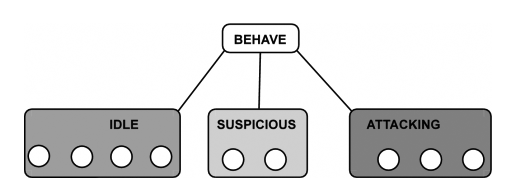
\includegraphics[scale=0.4]{images/btgen.png}
            \caption{A Tree of modular Behaviors~\cite{understandingbts}}
            \label{img:btgen}
            \end{center} 
        \end{figure}
        
        These behavior tasks are formally constructed out of 2 classes of constructs\footnote{As such, these constructs are also referred to as \textbf{tasks} or \textbf{task nodes}}. The Primitive constructs form the leaves of the tree, and define low level actions which describe the overall behavior. The composite constructs provide a standard way to describe relationship between children nodes, such as whether all should be executed or only a subset of them. In the next section, we cover these constructs, describing in detail their usage and applicabilities.
        
        \subsection{Primitive Constructs}
            
            % \subsubsection{Primitve Constructs}
            
            Primitive Constructs form the leaves of a Behavior Tree, and they define low-level basic actions. In Game AI, they are esentially the interface between the AI logic and the main game, and are wrappers over function calls that are used to execute an action within the game world, or query the state of the game. 
            
            \subsubsection{Actions and Conditions}
                
            Two primitive constructs consist of 2 types, namely,           
            
            \begin{enumerate}
            \item \texttt{Actions} - which cause an execution of methods or functions on the game world, e.g. Move a character, Decrease health, ...
            \item \texttt{Conditions} - which query the state of objects in the game world, e.g. Location of character, Amount of Health points, ...
            \end{enumerate}        
       
            These actions and conditions form the definitions of behavior tasks. For example, in Figure \ref{img:primitives}, we define a Behavior Tree task \textsc{Deduct Money From Player}. 
             
            \begin{figure}[h]
                \begin{center}
                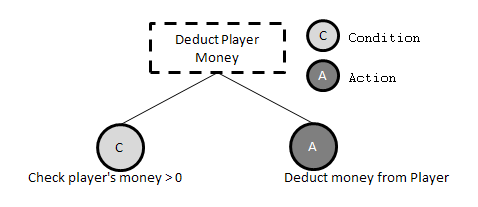
\includegraphics[scale=0.5]{images/primitives.png}
                \caption{A Behavior Task - Deduct Money From Player}
                \label{img:primitives}
                \end{center}            
            \end{figure}     
            
            \noindent The main task is decomposed into two child tasks, the left child being a \texttt{Condition} that the player has money to start with, and the right child being an \texttt{Action} which physically deducts the money from the player in the game. Each of these actions and conditions can either succeed or fail, which in turn define whether the high-level behavioral task succeeds or fails. 
                        
            \newpage
            
            \subsection{Composite Constructs}
            
            Now that we have introduced the notion of tasks, and how conditions and actions are used as child nodes to define these tasks. However, behavior tasks of these sorts are limited to very basic tasks. We are interested in increasing the complexity of these behavior tasks and this is achieved by building branches of the tree to organise the children nodes. These branches are essentially the composite constructs of behavior trees, and their main purpose involves organising the children nodes of each task. The composite tasks consist of,
            
            \begin{enumerate}
            \item \texttt{Sequences} 
            \item \texttt{Selectors} 
            \item \texttt{Decorators}
            \end{enumerate}
            
                    
            \subsubsection{Sequences}
            
            \begin{figure}[h]
                
                \begin{center}
                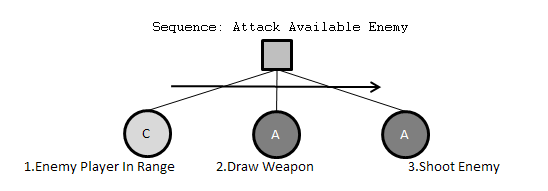
\includegraphics[scale=0.5]{images/sequence.png}
                \caption{Sequence Example - Attack Available Enemy}
                \label{img:sequence}
                \end{center}            
            \end{figure} 
            
            Figure \ref{img:sequence} shows a \texttt{Sequence} node, consisting of 3 children nodes, each being a primitive type. A \texttt{Sequence} essentially imposes an ordering on the execution of its children nodes. 
            
            In this example, it first checks if there is an enemy in range. Secondly, it draws a weapon before finally attacking the enemy. Note that the order of execution is important, since logically, a weapon has to be drawn before it can be used to fire at an enemy. Thus, in order to determine if the entire \texttt{Sequence} has executed successfully, each one of its children nodes has to execute successfully in the order that they are specified. 
            
            If in the event that an enemy is present, but the AI player does not have a weapon to draw, the second child task node fails, resulting in an automatic failure of the entire \texttt{Sequence}. The third child node, in this case, does not need to be checked or executed. Sequences can be seen to perform implicit pre-condition checking to prevent potentially unexpected behavior from occuring ( i.e. an AI player attempting to shoot before drawing a weapon ).
                        
            \subsubsection{Selectors}
            
            \begin{figure}[h]
                
                \begin{center}
                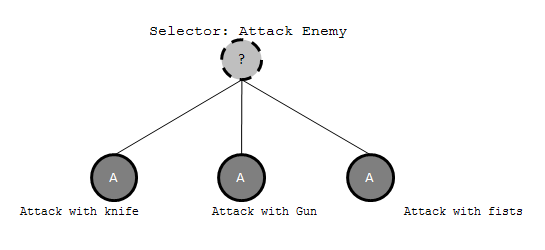
\includegraphics[scale=1.0]{images/selector.png}
                \caption{Selector - Attack Enemy}
                \label{img:selector}
                \end{center}            
            \end{figure} 
            
            The second type of composite we introduce is the \texttt{Selector}. Figure \ref{img:selector} shows a \texttt{Selector} node, consisting once again of 3 children nodes. The first thing to notice is that there exists no formal ordering on these children nodes. The reason is because, a \texttt{Selector} essentially chooses, or picks, one of its children nodes to be executed. This child node can be selected randomly, probalistically, or using priorities. For this example, we assume that each child node has an equal probability of being selected.

            On execution of a child node, the \texttt{Selector} succeeds only if at least one of its children nodes succeed. In our example, the game AI selects from 3 alternatives to complete the task \textsc{Attack Enemy}. If it first picks \textsc{Attack with Gun}, the corresponding \texttt{Action} executes. Supposing the \texttt{Action} fails, perhaps due to the AI player not possessing a gun at this point, the \texttt{Selector} node does not immediately fail, but rather, it picks a next child node to execute. 
            
            Continuing with our example, supposing the next \texttt{Action} it picks is \textsc{Attack with knife}. Assuming the AI player possesses a knife at this point and executes the action successfully, the \texttt{Selector} node then returns as successful. The \texttt{Selector} only fails when none of its children execute successfully. This can be seen as exhibiting an opposite behavior to that of \texttt{Sequences}.
            
            Sometimes, we assign priorities to each of the child task nodes. A \texttt{Selector} that selects its child task nodes in the order of decreasing priority is termed a \texttt{Priority Selector}.
            
            \subsection{Decorators}
            
            We have so far seen primitive and composite tasks which are used to design and define our Behavior Trees. \texttt{Decorators} are a class of tasks inspired by the software design pattern of the same name. Just as how Decorators in sofware design aim to wrap over an existing class, adding additional features on top of, but without modifying, the existing class, Behavior Tree \texttt{Decorators} aim to extend existing defined Behavior Trees to improve its functionality. 

            This is best illustrated with an example - consider the Behavior Tree in Figure \ref{img:sequence}. Supposing that in order to achieve a more realistic AI, we want the AI player to exhibit this \textsc{Attack Available Enemy} behavior for only a certain duration of time within the game, such that there are points when the AI player is considered "off-guard", to mimic how a human player would not always choose to attack an enemy even though one were present.
            
            \begin{figure}[h]
                
                \begin{center}
                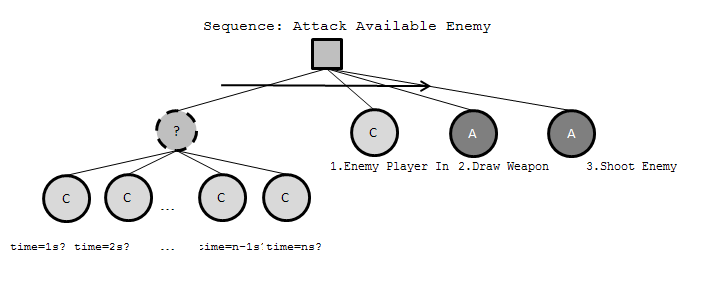
\includegraphics[scale=1.0]{images/badexample.png}
                \caption{An approach to handling timed behaviors}
                \label{img:badexample}
                \end{center}            
            \end{figure} 
            
            If we were to try to design a Behavior Tree to exhibit this behavior, we could try modifying our existing Behavior Tree to include several more \texttt{Condition} tasks linked together by a \texttt{Selector} into the existing \texttt{Sequence}, with each \texttt{Condition} checking for specific points of time within the game, such as in Figure \ref{img:badexample}. 
            
            This, however, can be seen to be undesirable on three accounts. Firstly, it breaks the simplicity of designing Behavior Trees because of the need to tediously create multiple \texttt{Condition} nodes. Next, this is definitely not scalable because if we were to increase the time duration to execute this behavior, more \texttt{Condition} tasks have to be added. Lastly, it breaks the rule of modularity since we are unable to reuse this Behavior for a different time duration other than that covered by the existing \texttt{Conditions}.
                       
            \texttt{Decorators} are thus the solution to this problem. What occurs is that we define a type of \texttt{Decorator} - a \texttt{Timer}, which executes it's child node for a specified duration of time. The existing behavior does not need to be modified in any way, except that the \texttt{Timer Decorator} is linked as the parent to the existing Behavior Tree, as depicted in Figure \ref{img:timer}. Now, the Behavior is simple to create because it only involves the addition of a single \texttt{Decorator Timer}, and maintains its modularity since the original behavior of \textsc{Attack Available Enemy} has not been modified in any way. Scalability does not pose a problem since there are no additional nodes to add.
            
            \begin{figure}[h]
                
                \begin{center}
                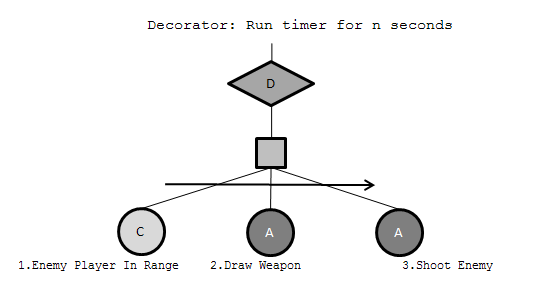
\includegraphics[scale=0.6]{images/decorator.png}
                \caption{Using timer decorators to handle timed behaviors}
                \label{img:timer}
                \end{center}            
            \end{figure}  

            This exhibits the usefulness of \texttt{Decorators} to extend the functionality of Behavior Trees, and more examples of types of \texttt{Decorators} include \texttt{Counters} which track and execute behaviors a certain number of times or \texttt{Debug Decorators} which output information about the corresponding child tasks. A non-exhaustive list of different types of \texttt{Decorators} can be found on page \pageref{app:decorators} of the Appendix.
            
            \subsubsection{Lookup Decorators}
            
            From the above discussion on \texttt{Decorators}, one noticeable point is that \texttt{Decorators} never appear as the leaves of a Behavior Tree, since their functionality essentially depends on their children tasks. However, one type of \texttt{Decorator} always appears as a leaf node and that is the \texttt{Lookup Decorator}, or \texttt{Lookups}. 
            
            \texttt{Lookups} attempt to further increase the modularity and reusiblity of Behavior Trees by using such \texttt{Lookups} to search for particular sub-behavior tasks rather than explicitly stating them in the tree. This can be illustrated by first considering the Behavior Tree in Figure \ref{img:lookup1}, describing a behavior of an AI player in the game of Defcon in the midst of placing a structure.
            
            \begin{figure}[h]
                
                \begin{center}
                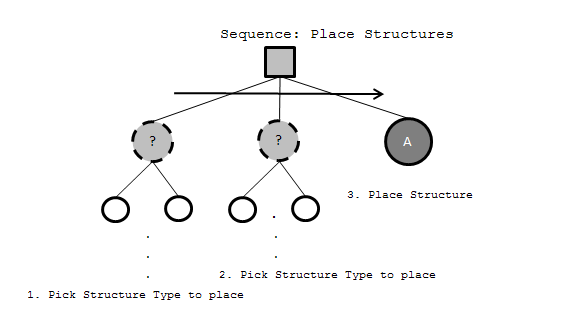
\includegraphics[scale=0.6]{images/lookup1.png}
                \caption{Behavior for AI Placing Structures in DEFCON}
                \label{img:lookup1}
                \end{center}            
            \end{figure}
         
            
            The Behavior takes the form of a \texttt{Sequence}. First it picks a structure to place, then it decides on a location for the structure and finally, it places it. The first two tasks involve \texttt{Selectors}, basically because we might design the AI in such a way that it has different implementations of deciding which structure to place. An example would be picking the structure that has the fewest remaining number or an alternative could be picking one with the highest remaining number. Similarly for the second task, we have different implementations from which we wish to select from in deciding the location to place the structure. For example, placing structures nearer the sea areas, closer to cities or closer together.
            
            Now, it can be seen that we are not interested from a high level perspective about the sequence of actions which are required to execute the different implementations of these tasks, we merely want the behavior tree to decide for us and accomplish the tasks \textsc{Pick Structure Type to Place} and \textsc{Pick Location to Place}. The idea is then to associate these different implementations into a lookup table, grouped by their high-level task which they are accomplishing, and replace the children nodes of the main \texttt{Sequence} by \texttt{Lookup Decorators}, as shown in Figure \ref{img:lookup2}.
                                   
            \begin{figure}[h]
                
                \begin{center}
                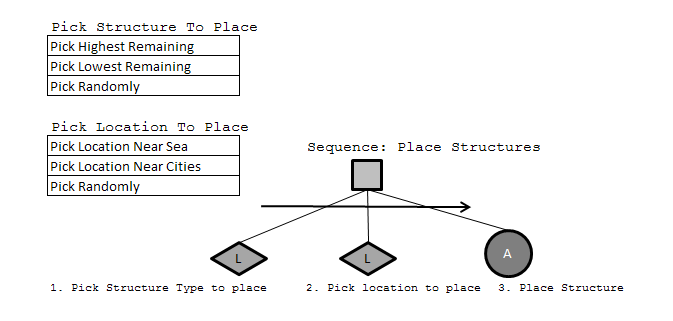
\includegraphics[scale=0.6]{images/lookup2.png}
                \caption{Using Lookups to modularise Behaviors}
                \label{img:lookup2}
                \end{center}            
            \end{figure}
            
            In grouping these implementations, into a hierarchy of tables, we begin to move towards a hierarchical goal-oriented architecture. These high-level tasks can be viewed as high-level goals which the Behavior ultimately wants to achieve, and does so by decomposing down to smaller sub-goals in order to achieve the high level goal. In Section \ref{sec:bod}, we discuss a theoretical methodogy of architecting game AI in what is called \textbf{Behavior Oriented Design (BOD)} \cite{bod}, and then propose our implementation of using Behavior Trees for the game of DEFCON to approach BOD.
            
            The idea of using \texttt{Lookups} to search for possible different sub-behaviors in a goal-oriented manner forms the basis of the idea of performing Planning in AI using Behavior Trees. In brief terms, planning involves the selection and sequencing of related actions from a given initial state to a target state. Its applicabilities to Behavior Trees and a description of how we chose to allow the Behavior Trees for DEFCON to exhibit planning is described in greater detail in Section \ref{sec:reactiveplanning}, 
            
    \newpage    
        \section{Behavior Oriented Design}
        \label{sec:bod}
        
        Behavior Oriented Design (\textbf{BOD}) is a development methodology proposed by Joanna Bryson \cite{bod} which aims to design and construct what are termed as \emph{complete complex agents}(\textbf{CCA}) in a modular fashion. The methodology serves as an improvement over current arhitectures for these \textbf{CCA}. In this section we provide an overview of \textbf{BOD}, its proposed approach to designing an AI which focuses on iterative rapid prototyping and how such an architecture would allow the AI to exhibit functionality such as reactive planning, which we will show to be desirable when attempting to design an AI for a complex and dynamic AI.     
        
        What interests us most about \textbf{BOD} is its close correspondence with Behavior Trees, which we introduced in Section \ref{sec:behaviortrees}, such as the similar functionality of \text{BOD}'s \texttt{Action Patterns} and \texttt{Competences} to the \texttt{Sequences} and \texttt{Selectors} of Behavior Trees respectively. It can then be shown, based on this correspondence, that idea of planning for arises naturally for both \texttt{BOD} and Behavior Trees.
        
        As a result, we shall then present the approach, using a combination of these two concepts, that we use to essentially create a \textbf{BOD}-inspired goal oriented Behavior Tree AI architecture for the purpose of this project.
        
        \subsection{Methodology}
        
        Using Behavior Oriented Design, we approach a modular and behavior-oriented approach to coding the AI. This is achieved by \emph{Behavior Decomposition} - essentially breaking down the complex high-level behavior into smaller sequences or groups of sub-behaviors. The problem that arises often taking this approach is determining how exactly do we decide to decompose a behavior. For example, we might wonder how much decomposition is necessary, how many sub-behaviors is ideal to define the top-level behavior and also how complex should they be. BOD approaches this via a cyclic development process involving a set of guidelines for this decomposition.
        
        We present the two main aspects of this development process, namely the \emph{Initial Decomposition} and subsequent \emph{Iterative Development} as proposed by Bryson \cite{bod}. After which, we demonstrate how this approach was used to cover the design of the Behavior Trees for this project.
        
        \pagebreak
        
        \subsubsection{Initial Decomposition}
        \label{sec:init-decompose}
        
        \begin{enumerate}
            \item Specify at a high level what the agent is intended to do
            \item Describe likely activities in terms of sequences of actions. These sequences are the basis of the intial reactive plans
            \item Identify an initial list of sensory and action primitives from the previous list of actions
            \item Identify the state necessary to enable the described primitives and drives. Cluster related static elements and their dependent primitives into specifications for behaviors. This is the basis of the behavior library.
            \item Identify and prioritize goals or drives that the agent may need to attend to, This descrivbes the intial roots of the reactive plan hierachy
            \item Select a first behavior to implement.       
        \end{enumerate}
        
        The initial decomposition process can be seen to be goal-directed, with the initial task being the high-level goal that it intends to achieve, and the sequences of actions representing the execution required to achieve this goal. Several other AI methods bear similarities to this, such as Hierarchical Task Networks~\cite{htn} and Goal Trees~\cite{goaltrees}. Figure~\ref{img:htn} shows an example of a \textbf{HTN}, and it can be seen to bear the characteritics of \textbf{BOD}'s task decomposition. We shall soon present and see that Behavior Trees may also be designed to exhibit such goal-directed behaviors.
        
        \begin{figure}[htp]
          \begin{center}
            \begin{tabular}{|l|l|}
            \hline
                \subfigure[Top level task \textbf{Hour} decomposed into sequence of subtasks and actions]{\label{img:htn-a}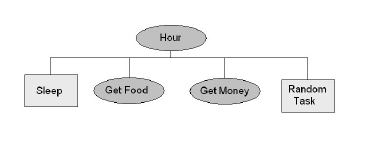
\includegraphics[scale=0.4]{images/htn_a.png}} &
                \subfigure[Sub-task \textbf{Get Food} is further decomposed ]{\label{img:htn-b}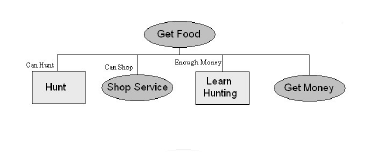
\includegraphics[scale=0.4]{images/htn_b.png}} \\ 
            \hline
            \end{tabular}
          \end{center}
          \caption{Hierarchical Task Network}
          \label{img:htn}
        \end{figure}
        
        \pagebreak
        
        The main motivation for such a goal-direct planning architecture arises from the second of two general philosophies of game AI \cite{actionprioritisation}. The first holds the belief that AI has to be strictly controlled using techniques such as finite automata like Finite State Machines and scripting. The reason for this is to give the AI developers a close control over the direction of the AI, what it is enabled to do in each state or situation and ultimately was to enable predictable behavior so as to ease the process of testing and debugging.
        
        The second philosophy, and the one which \textbf{BOD} pertains to, reasons that it is essentially impossible to adequately dictate and desribe every possible every possible action from every possible state. We have shown earlier that this is indeed true for Finite State Machines. Thus, it proposes that it is better to develop a reasoning AI that understands the basic rules of the game and makes its own decision based on the world as it perceives it, in hope that the emergent behavior would be more effective and believable than what could be specified by hand.
        
        \subsubsection{Iterative Development}
        
        The development process for the \textbf{BOD} methodology involves the following steps:
        
        \begin{enumerate}
            \item Select a part of the specification to implement next.
            \item Extend the agent with that implementation:
                \begin{itemize}
                    \item code behaviors and reactive plans, and
                    \item test and debug that code
                \end{itemize}
            \item Revise the current specification
        \end{enumerate}  
        
        \subsection{Goal-directed Reasoning}
        
        With both \emph{task decomposition} and the \emph{iterative development} process, we now highlight the approach undertaken in this project, using the \textbf{BOD} methodology to dictate the designing of the Behavior Trees for DEFCON's AI. In this section, we cover terms and ideas introduced in Section~\ref{sec:behaviortrees} and~\ref{sec:defcon}. We introduce the idea of \emph{goal-directed reasoning}, which is used in tandem with \textbf{BOD} for the construction of behavior trees
        
        \subsubsection{ Approach }
        
        The first thing to identify is the top-most goal that we want to achieve for our AI. Quite simply put, this top most goal would be to \emph{Win the Game}, and then we identify what are the sequences or groups of actions that this top level goal can be decomposed into, before recursively breaking down these subgoals down to primitive tasks such as \texttt{Actions} and \texttt{Conditions}. 
        
        This is an example of \emph{Goal-Directed Reasoning}, which is the opposite of another common methodology called \emph{Forward Reasoning}, which works by taking all the possible actions from a state, and applying each one to generate several subsequent states. This process continues until a target destination state is reached. This, however, is extremely cumbersome for a real-time strategy game such as Defcon, as the complexity of states and the unpredictibility of actions makes this approach prohibitive~\cite{goal-directed-reasoning}. 
        
        Goal-Directed Reasoning does the opposite, we identify a target goal state and then identify moves that might generate this goal state. The process is repeated for all predecessor states until the initial state is reached. An example of a planning procedure that employs this form of reasoning is the STRIPS approach~\cite{strips}.
        
        In Figure~\ref{img:deftoplevel}, we have identified our top most goal of our Behavior Tree to be, as we mentioned, \emph{Win the Game}. This is decomposed into 5 sub-goals which are named \emph{Defcon 5} to \emph{Defcon 1}. What this means is that, in order to achieve the top level goal of \emph{Win the Game}, we have to essentially \emph{Behave Optimally in Defcon 5}, \emph{Behave Optimally in Defcon 4}, ... and so on. This covers the first 2 steps of the \emph{initial decomposition} process introduced in Section~\ref{sec:init-decompose}. Note that we group these set of Defcon goals with a \texttt{Selector} node rather than a \texttt{Sequence} node, because we want the AI to choose the associated Defcon plan for each Defcon state the game is in. Using a \texttt{Sequence} would make the Behavior Tree fail once the game has proceeded to Defcon 4, and is not the correct behavior we wish to exhibit.
        
        \begin{figure}[h]                
            \begin{center}
            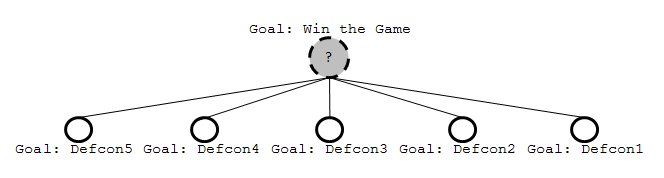
\includegraphics[scale=0.5]{images/defhighlevel.png}
            \caption{The Goal-Oriented Behavior Tree with its initial decomposition }
            \label{img:deftoplevel}
            \end{center}            
        \end{figure}
        
        Now, taking a look at these sub-goals which we have identified, we identify the need for a sensor primitive, or in Behavior Tree terms, a \texttt{Condition} task node, that performs a conditional check of the current Defcon state of the game. From here, we group these different sub-goals by registering them with Lookup Tables, which as we introduced, are used to group and modularize the Behavior Trees into a hierarchy, and we may later use  \texttt{Lookup Decorators} to locate these trees to enable reusability. This essentially covers steps 3 and 4 in Section~\ref{sec:init-decompose}. Figure~\ref{img:defnextlevel} shows the original tree now including the \texttt{Condition} nodes for each branch, as well as the grouping of them into a Lookup Table. Do note that the proposed Behavior Library essentially is the collection of Lookup Tables that we possess.
        
        \begin{figure}[h]                
            \begin{center}
            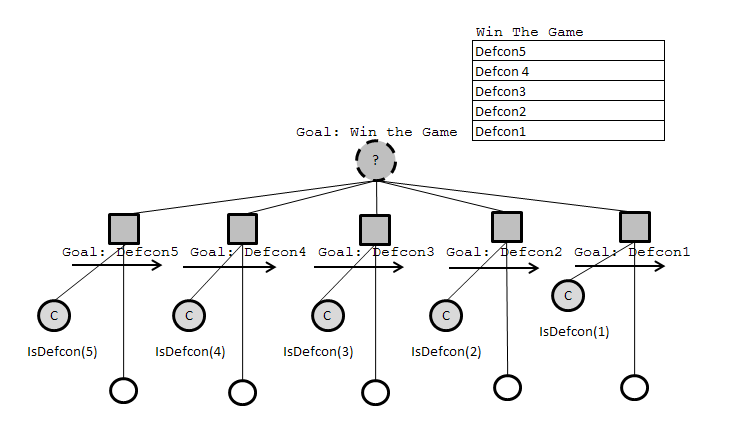
\includegraphics[scale=0.4]{images/defnextlevel.png}
            \caption{Each sub-goal introduces a set of primitives and other subgoals }
            \label{img:defnextlevel}
            \end{center}            
        \end{figure}
        
        Finally, as we mentioned, the use of Selectors was required to accomplish steps 5 and 6. Priorities are assigned to each branch corresponding to each Defcon state, and we assign a higher priority to \emph{Defcon 5} and continue in a decreasing order towards \emph{Defcon 1}, since at the start, we always begin in Defcon 5. This concludes the initial decomposition of the task \emph{Win the Game}. 
        
        \subsubsection{Subsequent Iterations}
        
        With the completion of the initial decomposition, we essentially test to ensure that all new introduced nodes are working correctly before moving on to the next phase of the iteration. A similar process is then replicated for each subgoal, decomposing the task further into subtasks until we reach a point when further decomposition is no longer permissible, which in the case of Behavior Trees, is when we have reached the leaves of the tree where only primitive task nodes exist. We now present the complete behavior tree of one of the branches, namely \emph{Defcon 5}, which was constructed for the purpose of the project. 
        
        \pagebreak
        
        \begin{figure}[h]                
            \begin{center}
            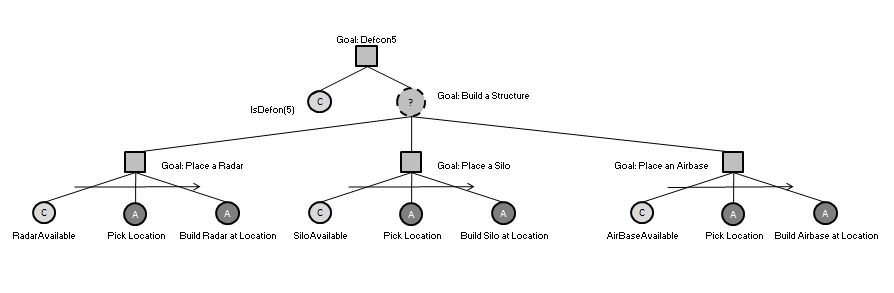
\includegraphics[scale=0.45]{images/defcon5.png}
            \caption{Complete Behavior Tree for Task: Defcon5}
            \label{img:defcon5}
            \end{center}            
        \end{figure}
        
        Figure~\ref{img:defcon5} above shows the complete behavior tree for the \emph{Defcon5} task. As we can see, the entire task consist of a sequence of actions. First, it checks whether the current DEFCON state of the game is DEFCON 5 using \textbf{Condition} \emph{IsDefcon(5)}. Next, it picks a structure type to place within the game world, leaving the choice randomly to the \texttt{Selector} \emph{Build a Structure}. This task is broken down into 3 sub-tasks.
        
        In order to place a structure, what involved is a \texttt{Sequence} first checking if there exist any available sturctures of the chosen type to be placed with a \texttt{Condition}. Next, it performs as \texttt{Action} to choose random coordinates to place the structure. Finally, upon picking the location, the AI proceeds to place the structure at the designated location with yet another \texttt{Action}.
        
        During the designing of the task \emph{Defcon5}, we have identified both the composites required, but more importantly, the primitive task nodes that are required to be constructed. These nodes, \emph{IsDefcon}, \emph{PickLocation} and \emph{Build Structure at Location} were identified as required primitives - which were then constructed and added into the list of actions and primitives for the entire AI. This process was repeated for each of the DEFCON tasks, and resulted in a cumulatively constructed library of primitive \texttt{Actions} and \texttt{Conditions}. The complete tree for the entire AI, covering all 5 DEFCON tasks can be found on page~\pageref{app:defconbts} of the Appendix.
        
        \newpage
        
        \subsection{Reactive Planning}
        \label{sec:reactiveplanning}
        
        In the previous section, we have described task decomposition in \textbf{BOD} and one importance of the ability to decompose our tasks is that by decomposing them down to simple enough subgoals, there arises the possibility of interleaving actions and tasks. This is possible for DEFCON, as a real-time strategy game due to its unpredictability of the game state due to the dynamic set of choices that both an AI and human player may execute. Overcoming this unpredictability by having this form of task decomposed interleaving is a form of \textbf{Reactive Planning}~\cite{goal-directed-reasoning}. This reactive planning is described in \textbf{BOD} by \emph{Action Selection}, and shows advantage over traditional architectures without similar support for reactive planning such as the Subsumption Architecture or Agent Network Architecture~\cite{bod}. We shall cover plan elements which \textbf{BOD} introduces to support \emph{action selection} in such reactive plans, namely \textbf{Action Patterns} and \textbf{Competences}, and subsequently draw their respective correspondence to Behavior Trees and how they implement something similar to them.
        
        \subsubsection{Action Patterns}
        
        An \emph{action pattern} describes a sequence of primitives, where the primitives are either actions or sensory actions, and its usefulness include:
        
        \begin{itemize}
        \item Aiding the AI designer to keep the system as simple as possible, communicating clearly the expected behavior of the plan segment
        \item Allows for speed optimization of elements that reliably run in order.        
        \end{itemize}
        
        \begin{figure}[htp]
          \begin{center}
            \begin{tabular}[c]{|l|l|}
            \hline
                \subfigure[Action Pattern]{\label{img:seq-actpats-a}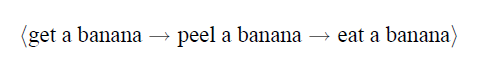
\includegraphics[scale=0.3]{images/bod-actpats}} &
                \subfigure[Sequence]{\label{img:seq-actpats-b}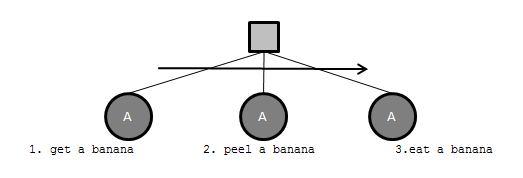
\includegraphics[scale=0.3]{images/seqbanana}} \\ 
            \hline
            \end{tabular}
          \end{center}
          \caption{Correspondence between Action Patterns and Sequences}
          \label{img:seq-actpats}
        \end{figure}
        
        We can see that \emph{action patterns} can be represented in Behavior Trees as \emph{Sequences}. Figure~\ref{img:seq-actpats} illustrates the this correspondence.
        
        \pagebreak
        
        \subsubsection{Competences}
        \emph{Competences} attempts to drop the temporal ordering of its group of actions in order to allow any of its elements to fire when in a perceptually equivalent context. Rather, a prioritization is assigned to each child action, shown in increasing order in the direction of the arrow. Preconditions are used to determine the executability of each element.
        
        \begin{figure}[htp]
          \begin{center}
            \begin{tabular}[c]{|c|c|}
            \hline
                \subfigure[Competence]{\label{img:sel-comps-a}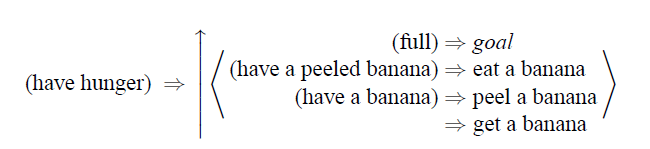
\includegraphics[scale=0.3]{images/bod-comps}} & 
                \subfigure[Selector]{\label{img:sel-comps-b}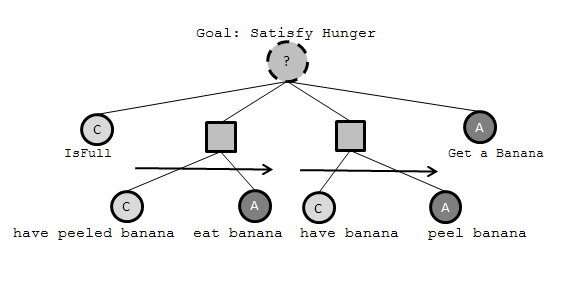
\includegraphics[scale=0.3]{images/selbanana}}  \\
            \hline
            \end{tabular}
          \end{center}
          \caption{Correspondence between Competences and Selectors}
          \label{img:sel-comps}
        \end{figure}
        
        Figure~\ref{img:sel-comps} shows the correspondence between \emph{Competences} and \texttt{Selectors}. It is worthwhile to note that the \texttt{Selector} in Figure~\ref{img:sel-comps-b} is a \texttt{Priority Selector} - where it places a priority values of decreasing value from left to right on its children task nodes.
      
       \subsubsection{Reactive planning for DEFCON fleets}
       
       Reactive planning provides a means for handling changes in the game world which cannot be pre-determined. One area in which this arises is in the coordination of the movement of fleets in DEFCON. For example, consider a fleet's movement from one point to another - during the length of its journey, an event, such as the detection of an enemy unit in the vicinity, might occur. We might want to be able to handle this by attempting to avoid the enemy by readjusting our route in such a way as to avoid the enemy. % optional: This is illustrated in Figure~\ref{img:avoiding}.
       
       Some AI approaches may find this problem difficult to handle. For example, the AI presented in Robin's thesis~\cite{robbot} does not actually handle this explcitly, instead, it the fleet will continue to move to its target destination as dictated by its plan. The unpredictability of such occurences makes this very difficult to plan for, and we require a solution that can perform a replanning at run-time.  This is where reactive planning comes in useful.
              
       \newpage
       
       \begin{figure}[h]                
                \begin{center}
                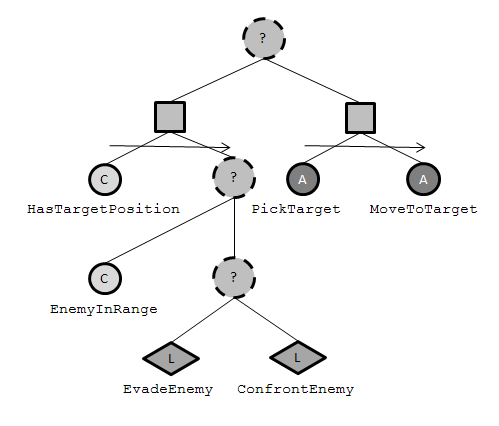
\includegraphics[scale=0.6]{images/movefleet.png}
                \caption{Behavior Tree to coordinate Fleet movement}
                \label{img:movefleet}
                \end{center}            
       \end{figure}
       
       In Figure~\ref{img:movefleet}, we present a behavior tree used to dictate the movement of a fleet. This tree can be seen as a replacement for the \emph{PatrolOrIdle} node for the behavior tree defined for \emph{Defcon4} on page~\pageref{app:d4} of the Appendix. At the top, we have a \texttt{Priority Selector}\footnote{We assume the convention that priority values of the children nodes decrease from left to right}, with two branches. In the left branch, we first check if the active fleet unit has a target position set. If not, the node fails, and the \texttt{Selector} chooses the right branch's node which picks a target destination and orders the fleet to move.
       
       Considering the left child's right branch now, we first check if any enemy has been detected within its radius in \emph{Enemy In Range?}. If none, no further action is required. But if we do detect an enemy, we then select whether to \emph{evade} or \emph{confront it} with yet another selector. 
       
       The behavior tree provides provides a way for a Fleet to proceed towards a target destination, but at the same time, allows it to handle the occurences of events easily by means of this form of reactive planning. For example, in the case where the the unit does not yet have a target destination, the sequence of actions would be:
       
       \begin{center}
       \texttt{ \scriptsize{ HasTargetPosition(Fail) -> PickTarget-> MoveToTarget} }
       \end{center}
       
       In the case where the fleet already has an active target, but no enemy is detected, we have:
       
       \begin{center}
       \texttt{ \scriptsize{ HasTargetPosition(Success) -> NoEnemyInRange(Sucess) } }
       \end{center}
       
       And in the final case, the fleet has an active target destination, and an enemy is detected during this time frame, we have:
       
       \begin{center}
       \texttt{ \scriptsize{ HasTargetPosition(Success) -> NoEnemyInRange(Fail)-> Evade} }
       \end{center}
       
       \emph{Evade} and \emph{Pursue} are assumed to have implementations defined in their respective behavior trees. Also, in this case, we assumed that \emph{Evade} had the higher priority, perhaps due to the AI's overall state of being defensive rather than offensive.
 
    \newpage
    
    \section{Genetic Algorithms} 
    \label{sec:ga}
        Designing an AI for a game is a complex task~\cite{actionprioritisation}, more so when developing one for a real-time strategy game like DEFCON, with its ever-changing game state, objects and their respective actions. One approach would be to hand-craft the AI based on the AI designers idea of what befits an appropriate AI, and such an approach would prove to be rather time-consuming in order to eventually produce an AI that is satisfiably robust. The AI designer would require to run through several iterations, each time changing or adding new states or variables to improve upon the AI of its previous iteration. The Introversion Bot of Section~\ref{sec:defcon-bots} is one such example.
        
        A second approach would be to introduce the ability of the AI to \emph{learn to play the game}~\cite{ml-and-games} via machine learning techniques. Machine Learning techniques have been successful in areas such as robotics~\cite{robotics}, and Robin's bot introduced in Section~\ref{sec:robbot} made used of \emph{case-based reasoning}, a form of machine learning technique 
        
        In this section, we introduce \emph{genetic algorithms} as our approach towards machine learning. We begin by formally introducing the terms and concepts of genetic algorithms. We then propose how they may be used as another key component of the development of DEFCON's AI for the purpose of this project.
        
        \pagebreak
        
        \subsection{Methodology}

        Genetic algorithms were inspired by the biological process of as \emph{evolution}. It serves to find near optimal solutions to complex non-linear problems~\cite{troll}, one such example being the designing of an appropriate AI for DEFCON. The approach usually begins by starting our with an initial population of solutions to the problems. These solutions are rated on how optimal they are, termed its \emph{fitness}, and subsequent populations are produced by a set of \emph{genetic oeprators}. This is allowed to repeat over numerous runs, or \emph{generations}, until a satisfactory performance is achieved. Informally, this can be desribed as a series of steps~\cite{mitchell}~\cite{troll}:
        
        \begin{enumerate}
            \item Create a first-generation of the population of random organisms
            \item Test them on the problem we are trying to solve, and rank them according to fitness. If the best organisms have reached our performance goals, stop.
            \item We produce the offspring organisms for the next generation via any combination of the following methods
            \begin{itemize}
                \item Carrying forward offsprings from the previous generation
                \item Producing new offsprings by genetic operators such as crossovers and mutation to the fittest individuals as identified in step 2
                \item Creating entirely new offsprings to introduce variety and prevent local maxima convergence
            \end{itemize}
            \item With this new set of individuals, we then repeat step 2.
        \end{enumerate}
                    
        \subsubsection{Implementation}
        
        The first step proposed above is to create the first-generation of the population of random organisms. In this case, each organism corresponds to each implementation of our AI bot using Behavior Trees. Each implementation can vary from one another by modifying the topology of the Behavior Trees or by maintaining the same topology and structure, but using a different set of values for the nodes in the tree. % optional: , and this is illustrated by means for Figure~\ref{img:first-gen
        
        Genetic algorithms can be applied both to find an optimal topology or optimal values for these nodes in the Behavior Tree. We first discuss the latter approach, where we present an approach to evolve our AI on one area of interest - the \emph{Optimal Placement of Silos}. We hope our AI to identify the best Silo placement positions in order to maximise its chance of success. We thus focus our attention to the \emph{Defcon5} branch of the our AI Behavior Tree which we constructed using the \textbf{BOD} process described in Section~\ref{sec:bod}. 

        \begin{figure}[h]                
                \begin{center}
                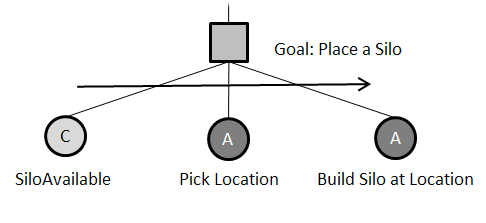
\includegraphics[scale=0.6]{images/placesilos.png}
                \caption{The Place Silo branch of Defcon 5's Behavior Tree}
                \label{img:placesilos}
                \end{center}            
            \end{figure}
        
        Figure~\ref{img:placesilos} above is from the middle branch of the \emph{Build a Structure} behavior tree from Figure~\ref{img:defcon5}. With this original implementation, the AI attempts to place a Silo at randomly picked coordinates, calculated by the \texttt{Action} node \emph{Pick Location}. Since the placement of structures for each player is only limited to their specific territory, there will be a chance that even if the \texttt{Condition} that a Silo is available to be placed, that the selected coordinates might end up being invalid. Thus, by running multiple runs of the game, we are able to generate a log file of valid and invalid coordinates for Silos as seen in Figure~\ref{img:silolog}.
    
        \begin{figure}[htp]
        \begin{center}        
        \begin{listing}{1}               
        InvalidLocation	Silo	-171.600006	76.900002
        InvalidLocation	Silo	-101.300003	95.699997
        InvalidLocation	Silo	-162.500000	-18.000000
        InvalidLocation	Silo	105.199997	-3.900000
        InvalidLocation	Silo	-77.900002	27.000000
        InvalidLocation	Silo	26.299999	88.800003
        ValidLocation	Silo	112.300003	29.200001
        ValidLocation	Silo	81.400002	31.000000
        ValidLocation	Silo	114.500000	41.000000
        ValidLocation	Silo	56.500000	31.600000
        ValidLocation	Silo	72.300003	37.000000 
        ValidLocation	Silo	53.799999	24.000000
        ValidLocation	Silo	102.199997	41.900002
        ValidLocation	Silo	83.300003	21.200001
        ValidLocation	Silo	109.400002	39.500000
        \end{listing}        
        \end{center}        
        \caption{Log of Valid and Invalid Silo placement positions for South Asia}
        \label{img:silolog}
        \end{figure}
        
        \subsubsection{Fitness}  
        
        \emph{Fitness} is a numerical measure of the performance of the organisms concerning the problem at hand. In this case, we may assign a simple fitness measure of each coordinate position by determining whether it was a valid or invalid placement location. However, it is important to consider several fitness functions, since incorrect convergence might occur~\cite{yaochu}. Some proposed fitness functions for the \emph{Placement of Silos} are,
                
        \begin{itemize}
        \item The amount of time the Silo managed to remain in the game, meaning that it was not destroyed.
        \item The number of enemy units it managed to destroy
        \item The number of successful nuclear hits on enemy buildings or units
        \end{itemize}
        
        These are just several proposed fitness function, and it would be interesting to investigate the results of applying each fitness function in this problem domain. There is also room to perhaps consider a combination of these fitness functions, using a simple~\emph{linear normalisation} method ~\cite{linearnorm}, but for the purpose of explanaining the following section on genetic operators in this report, we shall assume that only 1 fitness function is adopted.
   
        \subsection{Genetic Operators}
        Genetic operators are the set of operators that generate successors for each generation, producing a new population set for the next evolution iteration. 
        
        \subsubsection{Selection}
        
        \emph{Selection} involves picking a subset of the existing population to carry forward to the next generation. Three common forms of selection~\cite{mitchell} are
        
        \begin{itemize}
        \item Fitness Proportionate Selection
        \item Tournament Selection
        \item Rank Selection
        \end{itemize}
        
        In \emph{fitness proportionate selection}, individuals from the population are selected based on the ratio of its fitness to the fitness of the other individuals present in the current population. Thus, the probability of selecting an individual \texttt{x} from a population of \texttt{n} individuals is described by the equation,
        
        \begin{figure}[htp]
            \begin{center}
            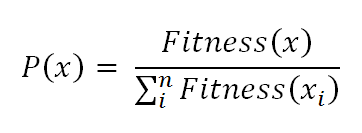
\includegraphics[scale=0.3]{images/eq_fitpropsel.png}
            \label{equ:fitpropsel}
            \end{center} 
        \end{figure}
        
        In \emph{tournament selection} involves first choosing at random two individuals from the existing population. The first is given a propability of \texttt{p}, and the second \texttt{(p-1)}.
        
        In \emph{rank selection}, the individuals are sorted according to their fitness. The probabilty of selecting an individual is then proprtional to its rank in this list, rather than its fitness.
       
        \subsubsection{Recombination}
        
        In recombination, two new individuals are generated for the next generation from two individuals from the existing population, termed as their parents. The aim of recombination is to allow the characteristics of the parents to be somewhat combined together, and thus, if we selected two parents with a high fitness, we would expect the offsprings to exhibit a hybrid of their characteristics and ideally, and improved fitness.
        
        We begin our explanation of recombination with an example, on the same topic of discussion as for the placement of silos. For the purpose of this explanation, all \texttt{Action} nodes are assumed to be \texttt{PlaceSilo(x,y)} nodes, where the arguments are labelled at each node.  Figure~\ref{img:recombination-a} is an example of \emph{single-point crossover}, where the dashed lines on the parent trees identify the point at which the recombination occured. From the diagram, it is clear to see that each offspring has a mixture of nodes from their parents. 
        
        \begin{figure}[htp]
            \begin{center}
            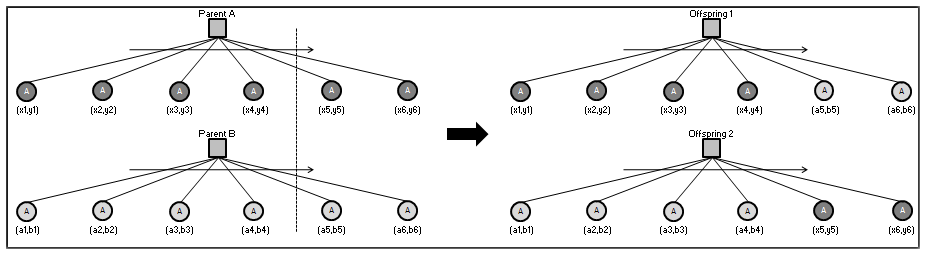
\includegraphics[scale=0.4]{images/recombination-a.png}
            \caption{Single-Point Crossover}
            \label{img:recombination-a}
            \end{center} 
        \end{figure}
        

        \pagebreak
        
        \begin{figure}[htp]
            \begin{center}
            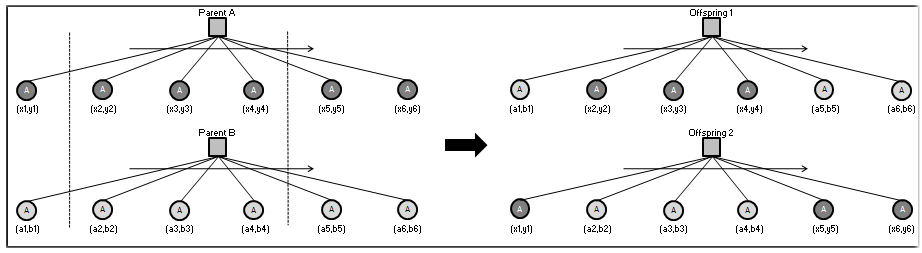
\includegraphics[scale=0.4]{images/recombination-b.png}
            \caption{Two-Point Crossover}
            \label{img:recombination-b}
            \end{center} 
        \end{figure}
        
        \begin{figure}[htp]
            \begin{center}
            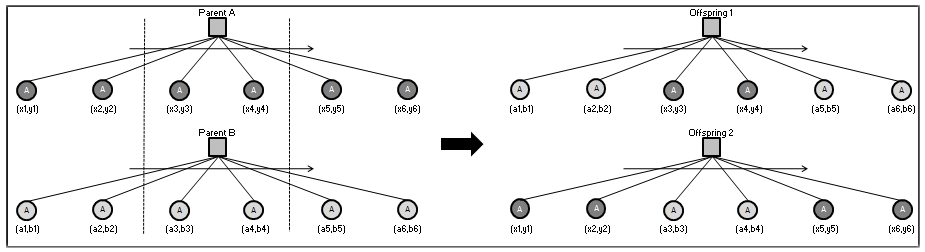
\includegraphics[scale=0.4]{images/recombination-c.png}
            \caption{Uniform Crossover}
            \label{img:recombination-c}
            \end{center} 
        \end{figure}
        
        Figure~\ref{img:recombination-b} shows offsprings generated when \emph{two-point crossover} was used. In this diagram, recombination occurs at two points, resulting in a greater mixture of nodes being passed from parent to offsprings. Figure~\ref{img:recombination-c} illustrates \emph{uniform crossover}, where the nodes are combined uniformly from the two parents.
                
        \subsubsection{Mutation}
        
        Mutations are employed to produce unpredictible random changes into individuals, modifying its attributes, so as to allow the individual to vary across generations. In this case, mutations can be useful to reintroduce placement coordinates that might have been lost or extinct due to being part of an unfavourable individual early in the evolution process. Mutations are also a good way to prevent against a local convergence, which tends to happen in small populations which very quickly become saturated with individuals that are locally optimal.
    
        \pagebreak
        
        \begin{figure}[htp]
          \begin{center}
            \begin{tabular}[c]{|c|}
            \hline
                \subfigure[Mutation by inserting new values]{\label{img:mutation-a}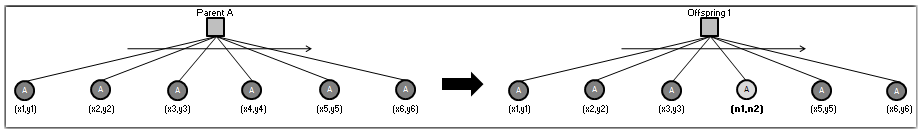
\includegraphics[scale=0.4]{images/mutation-a.png}} \\
                \subfigure[Mutation by modifying existing values]{\label{img:mutation-b}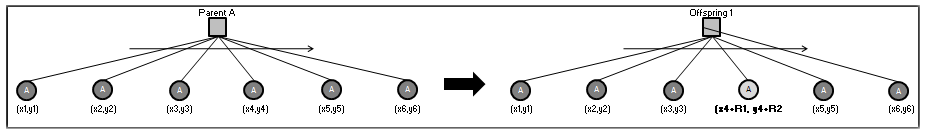
\includegraphics[scale=0.4]{images/mutation-b.png}}  \\ 
            \hline
            \end{tabular}
          \end{center}
          \caption{Mutations in Action nodes of Behavior Tree}
          \label{img:mutation}
        \end{figure}
        
        Figure~\ref{img:mutation} demonstrates mutation occuring for a node in the behavior tree. The coordinate values might be entirely regenerated, or perhaps, modified slightly. Figures~\ref{img:mutation-a} and ~\ref{img:mutation-b} illustrate this respectively.

        \subsection{Evolution Strategies}
        The previous sections have introduced genetic algorithms, genetic operators and how they may be used for the evolution of Bahavior Trees. We presented the evolution of the \emph{Placement of Silos} behavior trees using such an approach. We now present further areas of investigation of this evolution of behavior trees for the purpose of this project. 

        \begin{itemize}        
        \item Evolving the time of attacks for both units and structures
        \item Evolving the composition of fleets
        \item Evolving the placement and movement of fleets
        \end{itemize}

        \subsubsection{Evolving time of attacks}
        One key characteristic about the game of DEFCON is that the timing and coordination of an attack is crucial to winning~\cite{robbot}. A player who performs a well-coordinated and timed attack is more likely to do better than one who did random attacks sporadically throughout the game. We plan to investigate if, by the process of evolving these behavior trees, we are able to allow the bot to learn how to coordinate and time its attacks to maximise its score in the game. 
         
        \subsubsection{Evolving composition of fleets}
        In DEFCON, fleets present an area of significant interest. Firstly, the composition of fleets is highly variable, and we may investigate the implications of having different fleets of compositions. 

        \subsubsection{Evolving the placement and movement of fleets}
        Another interesting would concern the placement and movements of fleets. As mentioned in Section~\ref{sec:defcon}, some counties have two choices of sea territories to place fleets in. This, together with the target destination, has an impact as it may result in different lengths of time in order for a fleet to reach its target destination.

\chapter{Plan}
    
    This chapter provides information on the current state of the project at the approximate point of submission of this report. The chapter is divided into two sections:
    
    \begin{itemize}
    \item \textbf{Project Status}: Covers the current status of the project, implementation details and current AI ability.
    \item \textbf{Plan for Remainder of Project}: Covers plans for the remaining portion of thr project, classified in terms of weeks.
    \end{itemize}

    \section{Project Status}
    
    \subsection{Behavior Tree Design}
    
    For the purpose of this project, there was the necessity to develop a Behavior Tree data structure. Our implementation makes use of the \textbf{Composite Design Pattern} and the UML class diagram in Figure~\ref{img:uml_bt} shows our implementation. 

    \begin{figure}[h]                
        \begin{center}
            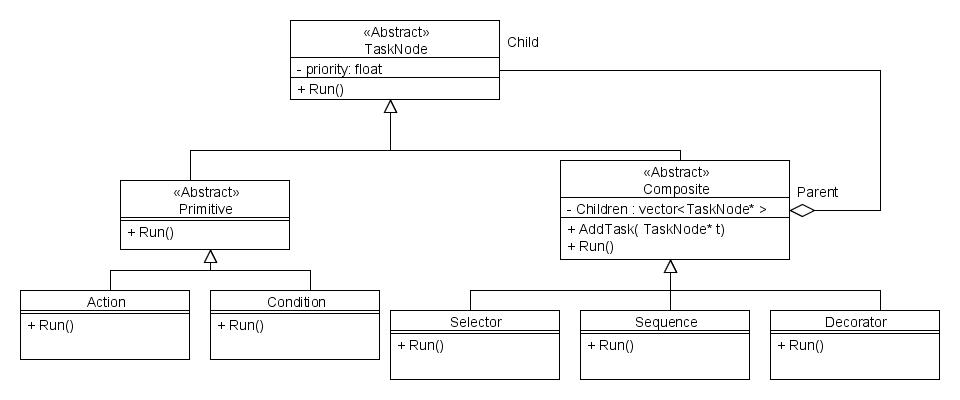
\includegraphics[scale=0.45]{images/uml_bt.jpg}
            \caption{UML Diagram for Behavior Trees}
            \label{img:uml_bt}
        \end{center}            
    \end{figure}
    
    \begin{itemize}
    \item The nodes of a Behavior Tree are of the \emph{abstract class}~\texttt{TaskNode}. 
    \item Two derived classes,~\texttt{Primitive} and~\texttt{Composite}, inherit from the~\texttt{TaskNode} class.
        \begin{itemize}
        \item Concrete classes~\texttt{Action} and~\texttt{Condition} are derived from~\texttt{Primitive}
        \item Concrete classes~\texttt{Selector},~\texttt{Sequence} and~\texttt{Decorator} are derived from~\texttt{Primitive}
        \end{itemize}   
    \end{itemize}    
    
    
    \subsection{System Design}
    
    The entire system consists of two main components - the DEFCON API and the Behavior Trees. As we can see from Figure~\ref{img:dependency}, the API's Bot class makes use of the Behavior Trees in order to execute AI logic and behavior. At the same time, the Behavior Trees need to be able to access the API calls to perform checks on the game state as well as executing commands. 
    
    \begin{figure}[h]                
        \begin{center}
        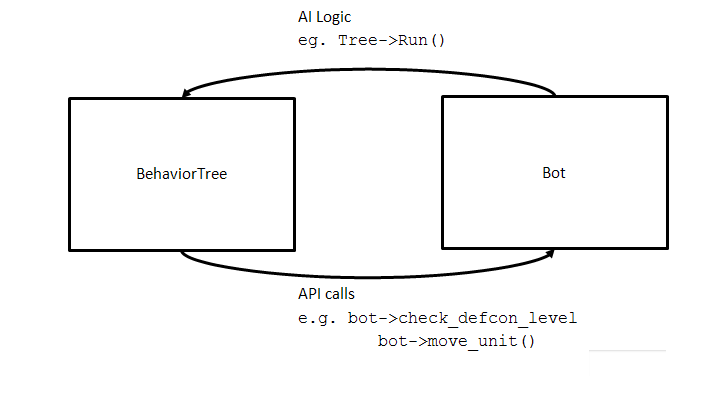
\includegraphics[scale=0.3]{images/dependency.png}
        \caption{Dependence of both the Behavior Tree and the Bot's API on each other}
        \label{img:dependency}
        \end{center}            
    \end{figure}
    
    \pagebreak
    
    Thus, in order to adhere to one of the core depency principles of having non-cyclic dependencies between classes, we have made use of the \emph{abstract client pattern}, which is illustrated by Figure~\ref{img:abstractclient}.
    
    \begin{figure}[h]                
        \begin{center}
            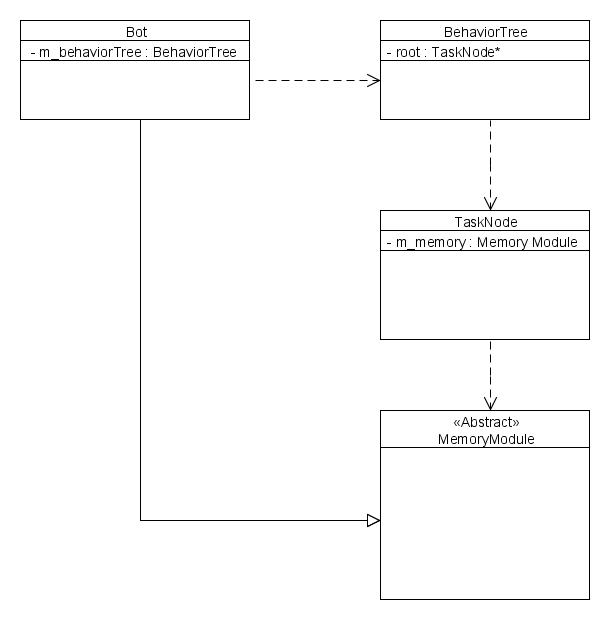
\includegraphics[scale=0.3]{images/uml_sysdesign.jpg}
            \caption{Abstract Client Pattern to prevent cyclic dependcies}
            \label{img:abstractclient}
        \end{center}            
    \end{figure}
    
    In this case, the Behavior Trees make use of what we term as a \textbf{MemoryModule} abstract class, and this essentially paves the way to to modularizing the Behavior Trees, make them reusable for any other application that may require it. For example, in the event a new game wanted to make use of the Behavior Trees, it would essentially ensure expose its API as a derived class of the MemoryModule abstract class, and create TaskNodes specific to that particular game.
    
    \newpage
    
    \subsection{AI Bot abilities} 

    At the point of writing, the AI is capable of playing the game of DEFCON, and more specifically, exhibits the following abilities:
    
    \begin{enumerate}
    \item Ability to place all 3 structure types - namely \textbf{RadarStations}, \textbf{Silos} and \textbf{AirBases}
    \item Ability to create and place fleets of any of the 3 naval forces types - \textbf{Battleships}, \textbf{Carriers} and \textbf{Submarines}
    \item Fleets are able to select a target destination and orders are sent for it to proceed to destination automatically.
    \item \textbf{Fighters} are launched to provide scouting at random locations
    \item Silos convert state to \textbf{Launch Mode} upon activation of DEFCON5, and target opponent cities.
    \end{enumerate}
    
    These abilities cover the main abilities, and allow the bot to perform actions throughout all 5 DEFCON levels. Target coordinates are now randomly picked by the bot, and in the next section we cover plans to improve upon this bot by evolving its behavior trees. 
    
    For reference, the behavior trees for each DEFCON level can be found in page~\pageref{app:defconbts} of the Appendix.
    
    \section{Upcoming Plans}
    
    The current abilities of the bot exhibits a naive players' approach to the game of DEFCON. The remainder of the project focuses heavily on improving upon this bot. More specifically, the evolving of the bots existing behavior trees, in hope of allowing the bot to gradually adapt and learn to play the game better. 
    
    A backlog of tasks pertaining to this project is included in page~\pageref{app:backlog} of the Appendix - which cover completed tasks, tasks in progress and tasks planned for the future. Here, we break down the plan into blocks of weeks, corresponding to the Department of Computing's calendar.
    
       
    \begin{center}
    \begin{tabular}{ | l | l | p{7cm}| }
    \hline
    \textbf{Term \& Week} & \textbf{Dates} & \textbf{Description} \\ \hline \hline
    Term 2 Week 06 & 15 FEB - 21 FEB & Begin evolution of Silo Placement. Submission of Interim Report. \\ \hline
    Term 2 Week 07 & 22 FEB - 28 FEB & Evolution of Silo Placement, working with Robin Baumgarten to refine API to allow collection of required data from DEFCON. Explore 2 fitness functions \\ \hline
    Term 2 Week 08 & 01 MAR - 07 MAR & Evolution of Fleet movement coordination, aim to get Fleets to identify "ideal" positions to place themselves for synchronised attack \\ \hline
      Term 2 Week 09 & 09 MAR - 14 MAR & Evolution of Aerial movement coordination. Aim to get Fighters to maximise fitness function or locating enemies, and Bombers to synchronise attacks \\ \hline
      Term 2 Week 10 & 10 MAR - 21 MAR & Coordinating evolved existing behaviors, aiming to combine abilities and provide global evolution of the AI \\ \hline
      Term 2 Week 11 & 22 MAR - 28 MAR & Collect preliminary statistics to assess current bot's abilities \\ \hline
      Easter Break & 29 MAR - 26 APR & Study break for examinations, code tweaking, refining and catch up on any implementation that was not able to be completed \\ \hline 
      Term 3 Week 01 & 26 APR - 02 MAY & Examinations \\ \hline
      Term 3 Week 02 & 03 MAY - 09 MAY & Examinations \\ \hline
      Term 3 Week 03 & 10 MAY - 16 MAY & Examinations \\ \hline
      Term 3 Week 04 & 17 MAY - 23 MAY & Assuming implementation working and performing desirably, begin work on reactive planning for fleet coordination \\ \hline
      Term 3 Week 05 & 24 MAY - 30 MAY & Work on reactive planning for Aerial coordination and movements \\ \hline
      Term 3 Week 06 & 31 MAY - 06 JUN & Consolidating report, findings and evaluation \\ \hline 
      Term 3 Week 07 & 07 JUN - 13 JUN & Consolidating report, findings and evaluation \\ \hline 
      Term 3 Week 08 & 14 JUN - 20 JUN & Final Report Submission \\ \hline
      Term 3 Week 09 & 21 JUN - 26 JUN & Presentation \\   
    \hline
    \end{tabular}
    \end{center}
    
    
      
    



%The Appendix
\chapter*{Appendix}
\addcontentsline{toc}{chapter}{Appendix}

    \section*{List of Decorators}
    \label{app:decorators}
        This presents a non-exhaustive list of proposed \textbf{Decorators} types, as suggested by Alex J. Champandard~\cite{btdecorators}.
        \begin{itemize}
        \item \textbf{Filters}: These prevent a behavior from activating under certain circumstances.
            \begin{itemize}
                \item Limit the number of times a behavior can be run
                \item Prevent a behavior from firing too often with a timer
                \item Temporarily deactivate a behavior by script
                \item Restrict the number of behaviors running simultaneously
            \end{itemize}
        \item \textbf{Managers \& Handlers}: These are decorators that are responsible for managing whole subtrees rather than single behaviors. 
            \begin{itemize}
                \item Deal with the error status code and restart planning or execution
                \item Store information for multiple child nodes to access as a blackboard            
            \end{itemize}
        \item \textbf{Control Modifiers}: These decorators are used to pretend that the execution of the child node happened differently
            \begin{itemize}
                \item Force a return status, e.g. always fail or always succeed
                \item Fake a certain behavior, i.e. keep running instead of failing or succeeding   
            \end{itemize}
        \item \textbf{Meta Operations}: Such decorators are useful during development, and can be inserted into a tree automatically when needed.
            \begin{itemize}
                \item Debug breakpoint; pause execution and prompt the user
                \item Logging; track this node execution and print to the console
            \end{itemize}        
        \end{itemize}
        
    \newpage
        
    \section*{Project Backlog}
    \label{app:backlog}
        \begin{figure}        
        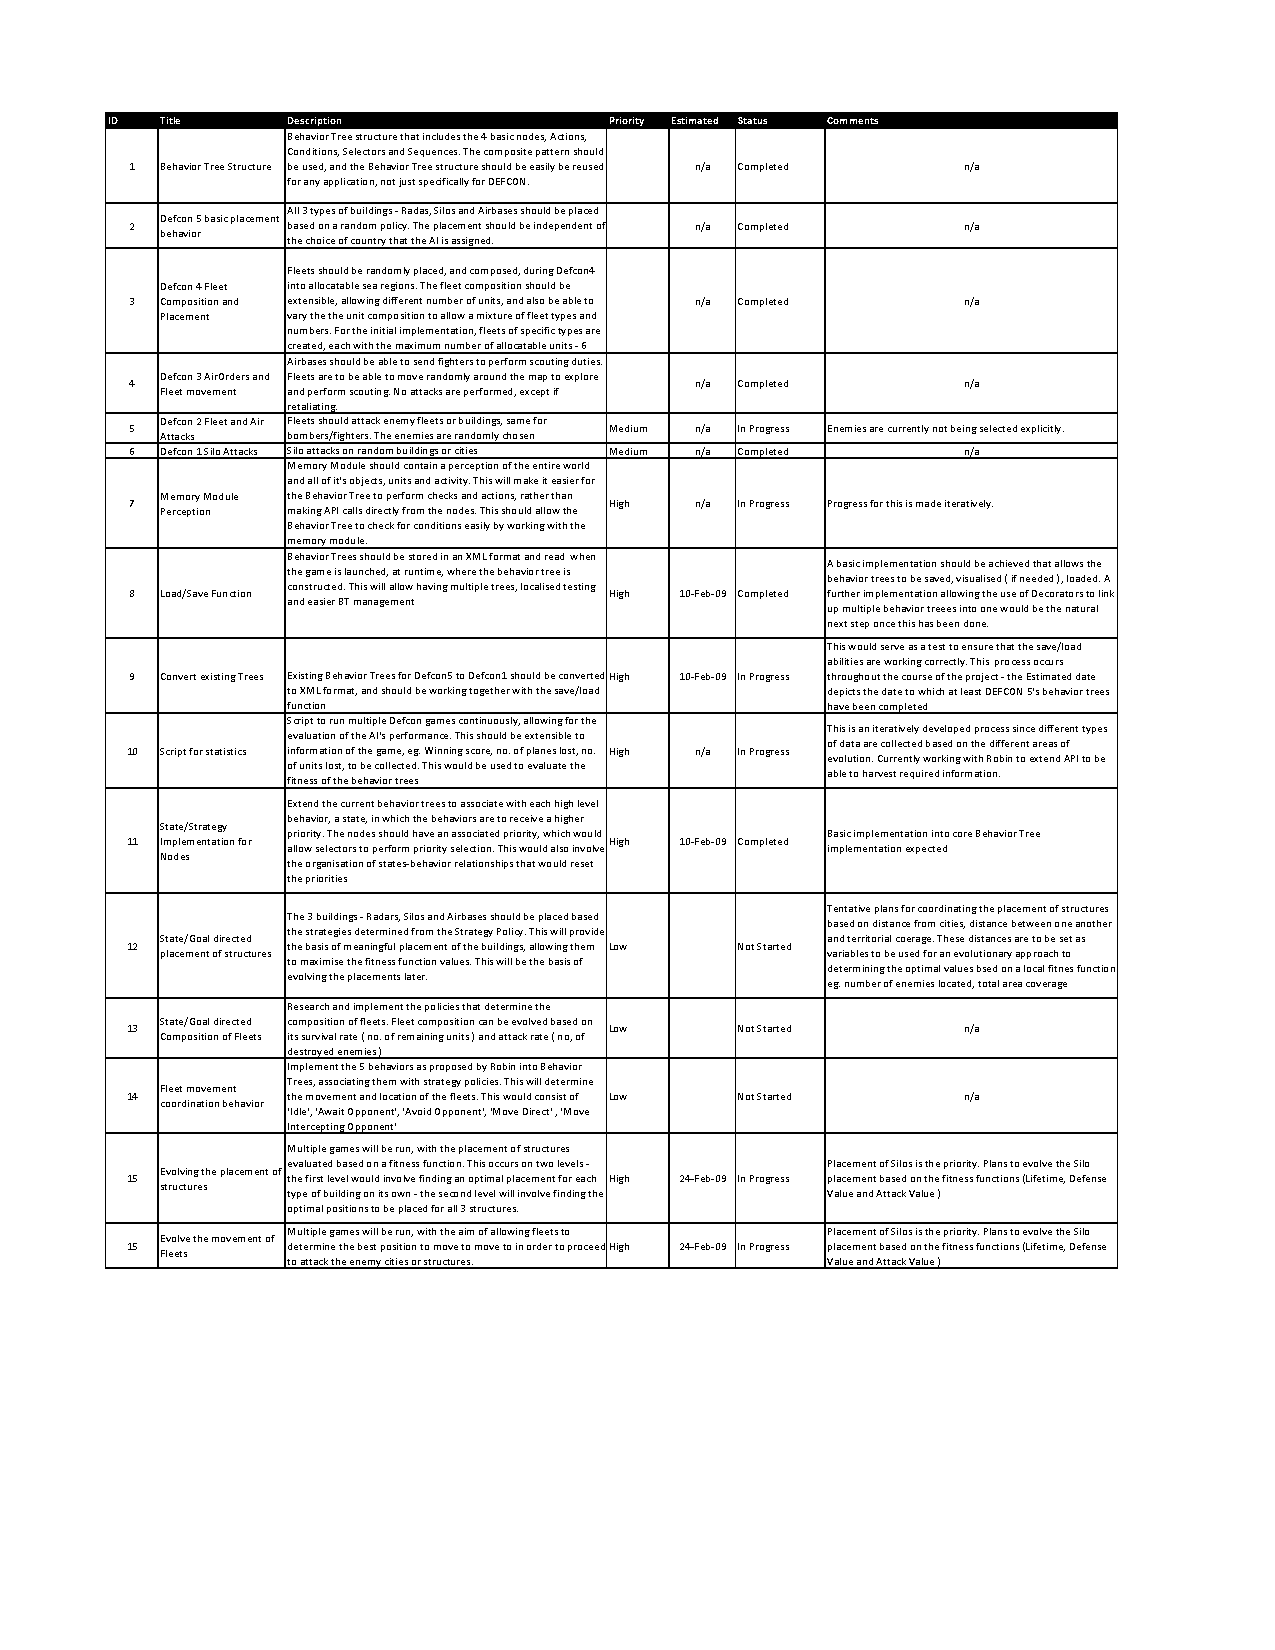
\includegraphics[bb=1.5in 2.0in 7.5in 9in,page=1]{backlog}
        \end{figure}
        
    \newpage
        
    \section*{DEFCON Behavior Trees}
    \label{app:defconbts}
    The tree diagrams here were automatically generated from the code. The nodes do not take the shape of the convention used in the report, instead nodes are prefixed to indicate the node types. The prefixes are:
    \begin{itemize}
    \item \textbf{ACT}: \texttt{Action} node
    \item \textbf{CON}: \texttt{Condition} node
    \item \textbf{SEL}: \texttt{Selector} node
    \item \textbf{SEQ}: \texttt{Sequence} node
    \item \textbf{PSEL}: \texttt{Priority Selector} node
    \end{itemize}
       
    \begin{figure}[h]
        \begin{center}
        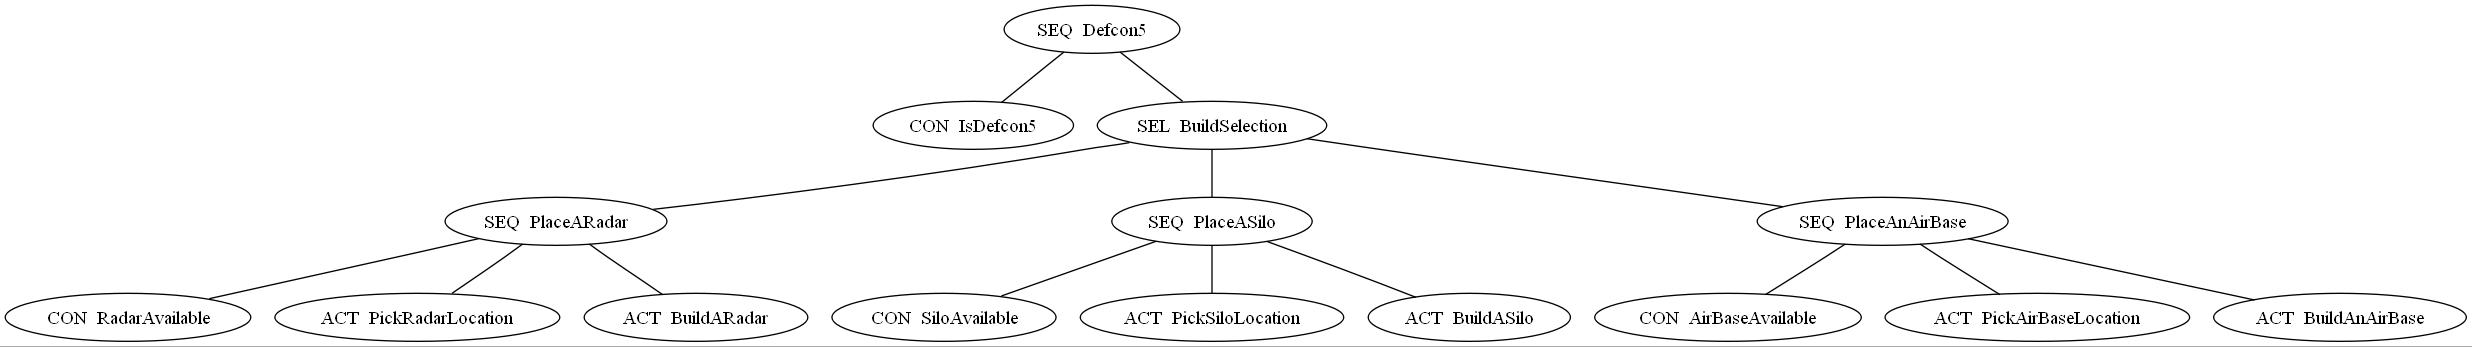
\includegraphics[scale=0.2, angle=270]{images/defcon5r.png}
        \caption{Defcon 5}        
        \end{center} 
    \end{figure}
    
    \begin{figure}[h]
        \begin{center}
        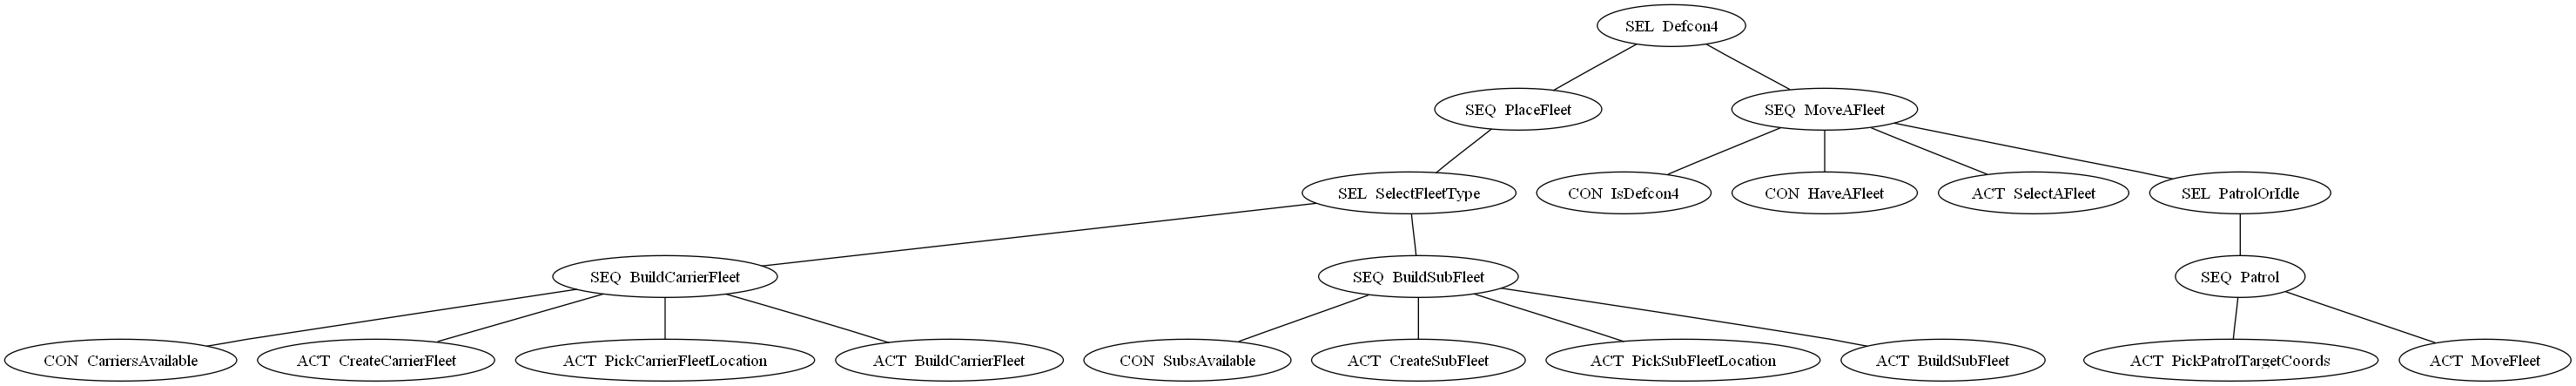
\includegraphics[scale=0.2, angle=270]{images/defcon4r.png}
        \caption{Defcon 4}  
        \label{app:d4}
        \end{center} 
    \end{figure}
    
    \begin{figure}[h]
        \begin{center}
        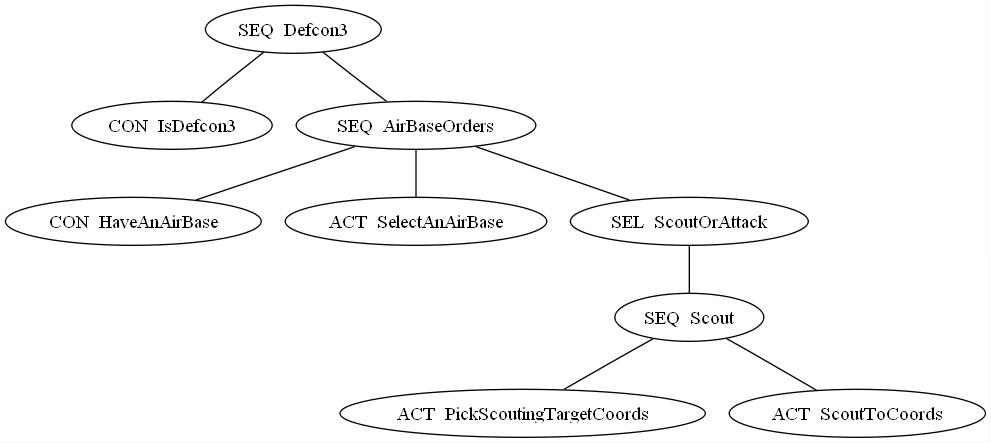
\includegraphics[scale=0.4]{images/defcon3r.png}
        \caption{ Defcon 3 and Defcon 2} 
        \end{center} 
    \end{figure}
    
    \begin{figure}[h]
        \begin{center}
        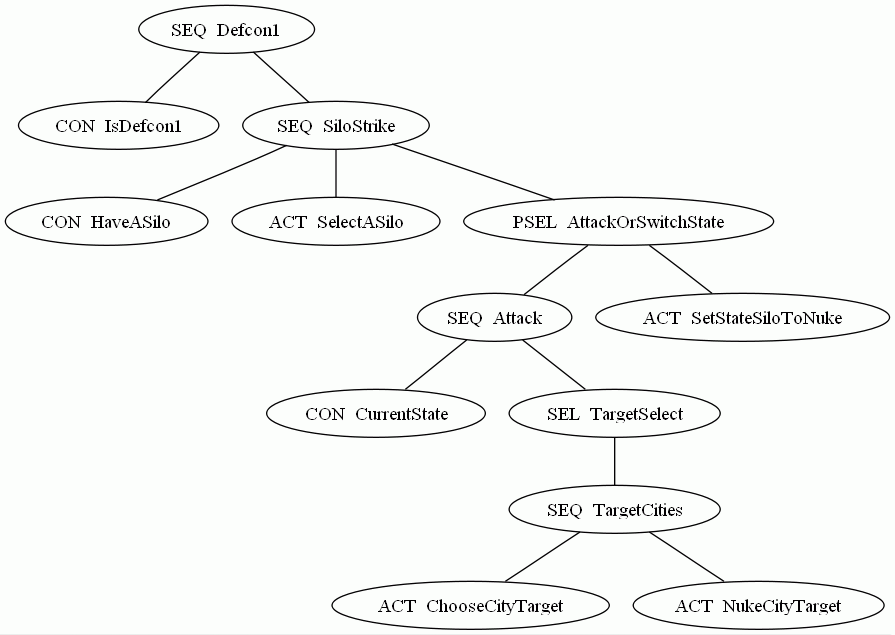
\includegraphics[scale=0.4]{images/defcon1r.png}
        \caption{Defcon 1}        
        \end{center} 
    \end{figure}


% The Bibliography
\bibliographystyle{alpha}
\nocite{*}
\bibliography{report_bib}\addcontentsline{toc}{chapter}{Bibliography}


\end{document}
